\documentclass[10pt,twocolumn]{article}
\usepackage[letterpaper,margin=0.75in]{geometry}
\usepackage{natbib}

\usepackage{fancyhdr}
\usepackage{lastpage}
\usepackage{microtype}
\usepackage{graphicx}
\usepackage{booktabs} % for professional tables
\usepackage{multicol}
\usepackage{multirow}
\usepackage{rotating}

\usepackage{tikz}
\usetikzlibrary{positioning}
\usepackage{titlesec}

\usepackage{mathtools}
\usepackage{amssymb}
\usepackage{amsthm}

\usepackage{hyperref}
\hypersetup{
  colorlinks=true,
  linkcolor=blue,
  citecolor=blue,
  urlcolor=blue
}
\usepackage[capitalize,noabbrev]{cleveref}

\usepackage{balance}
\usepackage[font=normalsize,labelfont=bf]{caption}

\usepackage{authblk}

% paragraph spacing + indent
\setlength{\parskip}{4pt plus 2pt minus 1pt}
\setlength{\parindent}{1.5em}

%%%%%%%%%%%%%%%%%%%%%%%%%%%%%%%%
% THEOREMS
%%%%%%%%%%%%%%%%%%%%%%%%%%%%%%%%
\theoremstyle{plain}
\newtheorem{theorem}{Theorem}[section]
\newtheorem{proposition}[theorem]{Proposition}
\newtheorem{lemma}[theorem]{Lemma}
\newtheorem{corollary}[theorem]{Corollary}
\theoremstyle{definition}
\newtheorem{definition}[theorem]{Definition}
\newtheorem{assumption}[theorem]{Assumption}
\theoremstyle{remark}
\newtheorem{remark}[theorem]{Remark}

%% Section adjustments, section spacing: {left}{before}{after}
\titlespacing*{\section}{0pt}{1.0ex}{0.4ex}
\titlespacing*{\subsection}{0pt}{1.6ex}{0.3ex}
\titlespacing*{\subsubsection}{0pt}{0.2ex}{0.2ex}

% --- Footer metadata ---
\newcommand{\leadauthor}{Booeshaghi \& Streets}
\newcommand{\repository}{bio\textcolor{red}{R}$\chi$iv}
% --- Page style ---
\pagestyle{fancy}
\fancyhf{} % clear all

% No header rule
\renewcommand{\headrulewidth}{0pt}
\renewcommand{\footrulewidth}{0pt}

% Footer text blocks
\newcommand{\LeftFooter}{%
 \footnotesize \leadauthor\ \textbar\ \repository\ \textbar\ \today%
}

\newcommand{\RightFooter}{%
  \footnotesize \thepage\ of \pageref{LastPage}%
}

% Two-sided safe (works for one-sided too)
% Works for one- or two-sided documents
\fancyfoot[L]{\LeftFooter}
\fancyfoot[R]{\RightFooter}

% Plain style (first page)
\fancypagestyle{plain}{%
  \fancyhf{}
  \fancyfoot[L]{\LeftFooter}
  \fancyfoot[R]{\RightFooter}
  \renewcommand{\headrulewidth}{0pt}
}


% two column space
\setlength{\columnsep}{18pt}

%% Author stuff
\date{}
\title{\textbf{Verifying LLM-extracted text with token alignment}}

\author[1]{A.~Sina Booeshaghi\thanks{Corresponding author: sinab@berkeley.edu}}
\author[1,2,3,4]{Aaron Streets}

\affil[1]{\small Department of Bioengineering, University of California Berkeley, Berkeley, USA}
\affil[2]{\small Center for Computational Biology, University of California, Berkeley, USA}
\affil[3]{\small Biophysics Graduate Group, University of California, Berkeley, USA}
\affil[4]{\small Chan Zuckerberg Biohub -- San Francisco, USA}
\setlength{\affilsep}{2pt}        % space between affiliation lines
% Center the affiliation block, but left-align its contents


\begin{document}

\twocolumn[
\begin{@twocolumnfalse}
\maketitle
\begin{abstract}
Large language models (LLMs) excel at text extraction, but they sometimes hallucinate. A simple way to avoid hallucinations is to remove any extracted text that does not appear in the original source. This check is easy for contiguous text, where exact string matching succeeds. Extracted phrases, however, are often non-contiguous---interrupted by punctuation, symbols, or parentheticals---and whether they can be found depends on how the text is tokenized. Using two new benchmark datasets, \texttt{BOAT} (derived from \texttt{SQuAD}) and \texttt{BIO-BOAT} (built from 51 bioRxiv preprints), we show that word-level tokenization recovers 53\% of held-out non-contiguous phrases, while any tokenizer that separates punctuation from words recovers over 99\%. We formalize alignment as a hierarchy of constraints and implement ordered alignment in \texttt{taln}, a tool that enumerates every order-preserving alignment with its source positions and selects among them with a simple rule that identifies a correct location first for 99.7\% of held-out phrases. An LLM given the same task produced verbatim evidence for 96.8\% of phrases and refused, misplaced, or miscopied the rest.
On 512 human-curated marker labels from seven single-cell studies, ordered alignment under subword tokenization recovered 99.8\%, and the failures that remained were differences of meaning rather than of matching.
\end{abstract}
\vspace{1em}
\end{@twocolumnfalse}
]

\section{Introduction}
Text extraction is a basic task for large language models (LLMs). A user asks the model to extract information from a passage, and the model is expected to return text that actually appears in it. Reliable text extraction is enabling. It allows users from many domains to turn unstructured text---such as a scientific article, historical newspaper, health record, or financial report---into structured data \citep{Gupta2022, Dunn2022, Agrawal2022, Kartchner2023, Huang2023, Dagdelen2024, Zhang2024, Polak2024, Chataut2024, Perot2024, Dagli2024, LeGuellec2024, Liu2024, Castro2024, Gartlehner2024, Pai2024, Ntinopoulos2025, Tang2025, Geevarghese2025, SchillingWilhelmi2025, Azar2025, Schwitter2025, Qin2025, Yamagishi2025, Srivastava2025, Jiang2025, Fei2025, zhou2025textminedataevaluationframework}.

In medicine and biology, accurate text extraction is especially important. For instance, organ procurement organizations rely on lab values and vital signs---often buried inside unstructured clinical notes---to judge whether a potential donor's organs are suitable \citep{Adam2025ClinicalExtraction}. Errors introduced during extraction can potentially misinform clinical decisions, and ultimately harm patients.

Fortunately, text extraction can be verified: we can align the extracted text back to its source (Figure~\ref{fig:example}). For uninterrupted (``contiguous'') phrases, verification is straightforward. An exact match confirms its existence. For non-contiguous phrases, verification is harder; alignment must handle intervening elements. Parenthetical notes, superscripts, symbols, qualifiers, or punctuation may interrupt a logically unified (but practically discontinuous) phrase. For example, the phrase ``\texttt{natural killer cells}'' in Figure~\ref{fig:example} cannot be contiguously aligned because the intervening parenthetical expression ``\texttt{(NK)}'' breaks it. Even though the phrase exists, it cannot be found by exact string matching. This situation is particularly acute in biology and medicine where non-contiguous phrases and non-standard nomenclature are highly abundant \citep{Lever2020NCS,Shinohara2024NCS}. 

\begin{figure*}[!t]
% color helpers
\newcommand{\tokenbox}[1]{\fcolorbox{black}{white}{\strut #1}}
\newcommand{\alntokenbox}[1]{\fcolorbox{green}{white}{\strut #1}}
\newcommand{\nalntokenbox}[1]{\fcolorbox{red}{white}{\strut #1}}
\centering
\fbox{%
  \parbox{0.975\textwidth}{%
    \textbf{Task:} Extract cell-type marker genes from the text below.\\[4pt]
    \textbf{Paragraph:} ``\dots Analysis of human immune cells from scRNA-seq and sNuc-seq samples again revealed expected cell types, including multiple subpopulations of monocytes, macrophages (CD14+), dendritic cells, B and T lymphocytes, and natural killer (NK) cells (CD96+), mast cells (CPA3+), and neutrophils (CSF3R+)'' \\[8pt]
    \textbf{Extraction}: \\
    Celltype: \textit{``natural killer cells''}, Gene: \textit{``CD96''}\\
    \dots\\

    % ---------------- PHRASE LEVEL ----------------
    \textbf{Task:} Verify the existence of the extracted cell-type marker genes.\\[4pt]
    \centerline{\textbf{Character alignment}}
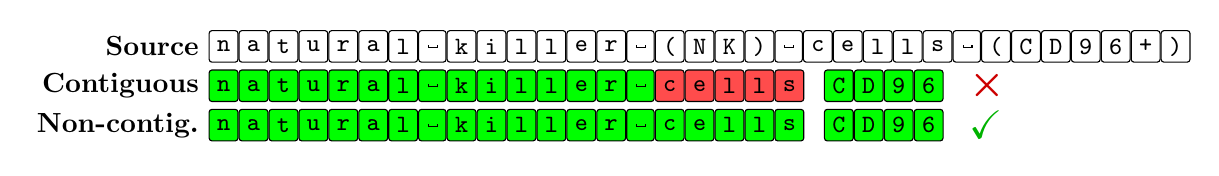
\begin{tikzpicture}[
  char/.style={
    draw, rounded corners=1pt,
    minimum height=4mm,
    inner xsep=1mm,  % horizontal padding inside variable-width boxes
    inner ysep=0pt,
    font=\ttfamily\small, align=center
  },
  idx/.style={font=\scriptsize, text=black!60},
  match/.style={dashed, thick, black!60}
]
\def\xgap{0mm} % gap between boxes

% --- Source ---
\node[anchor=east, font=\bfseries] at (0,0) {Source};

\foreach \c [count=\i] in {n,a,t,u,r,a,l,\textvisiblespace,k,i,l,l,e,r,\textvisiblespace,\symbol{40},N,K,\symbol{41},\textvisiblespace,c,e,l,l,s,\textvisiblespace,\symbol{40},C,D,9,6,+,\symbol{41}} {
  \ifnum\i=1
    \node[char, anchor=west] (s\i) at (0,0) {\c};
  \else
    \node[char, right=\xgap of s\the\numexpr\i-1\relax] (s\i) {\c};
  \fi
}

% --- Contiguous ---
\node[anchor=east, font=\bfseries] at (0,-0.5) {Contiguous};

\foreach \c [count=\i] in {n,a,t,u,r,a,l,\textvisiblespace,k,i,l,l,e,r,\textvisiblespace,c,e,l,l,s} {%
  % up to (and including) the space before "cells" is i<=15
  \ifnum\i<16
    \def\myfill{green}%
  \else
    \def\myfill{red!70}%
  \fi

  \ifnum\i=1
    \node[char, fill=\myfill, anchor=west] (t\i) at (0,-.5) {\c};
  \else
    \node[char, fill=\myfill, right=\xgap of t\the\numexpr\i-1\relax] (t\i) {\c};
  \fi
}

\node[anchor=west, font=\bfseries] (genelabel1) at (t20.east) {};

\foreach \c [count=\i] in {C,D,9,6} {
  \ifnum\i=1
    \node[char, anchor=west, fill=green] (g1\i) at (genelabel1.east) {\c};
  \else
    \node[char, right=\xgap of g1\the\numexpr\i-1\relax, fill=green] (g1\i) {\c};
  \fi
}
\node[anchor=west, font=\Large, text=red!80!black]
  at ([xshift=2mm]g14.east) {$\boldsymbol{\times}$};


% --- Non-contiguous ---
\node[anchor=east, font=\bfseries] at (0,-1) {Non-contig.};
\foreach \c [count=\i] in {n,a,t,u,r,a,l,\textvisiblespace,k,i,l,l,e,r,\textvisiblespace,c,e,l,l,s} {
  \ifnum\i=1
    \node[char, anchor=west, fill=green] (t\i) at (0,-1) {\c};
  \else
    \node[char, right=\xgap of t\the\numexpr\i-1\relax, fill=green] (t\i) {\c};
  \fi
}

\node[anchor=west, font=\bfseries] (genelabel2) at (t20.east) {};

\foreach \c [count=\i] in {C,D,9,6} {
  \ifnum\i=1
    \node[char, anchor=west, fill=green] (g2\i) at (genelabel2.east) {\c};
  \else
    \node[char, right=\xgap of g2\the\numexpr\i-1\relax, fill=green] (g2\i) {\c};
  \fi
}
\node[anchor=west, font=\Large, text=green!70!black]
  at ([xshift=2mm]g24.east) {$\checkmark$};

\end{tikzpicture}
    
    % ---------------- WORD-LEVEL ----------------
    \centerline{\textbf{Subword alignment}}
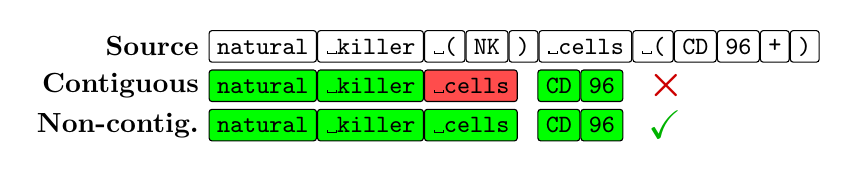
\begin{tikzpicture}[
  char/.style={
    draw, rounded corners=1pt,
    minimum height=4mm,
    inner xsep=1mm,  % horizontal padding inside variable-width boxes
    inner ysep=0pt,
    font=\ttfamily\small, align=center
  },
  idx/.style={font=\scriptsize, text=black!60},
  match/.style={dashed, thick, black!60}
]
\def\xgap{0mm} % gap between boxes

% --- Source ---
\node[anchor=east, font=\bfseries] at (0,0) {Source};

\foreach \c [count=\i] in {natural,\textvisiblespace killer,\textvisiblespace \symbol{40},NK,\symbol{41},\textvisiblespace cells,\textvisiblespace \symbol{40},CD,96,+,\symbol{41}} {
  \ifnum\i=1
    \node[char, anchor=west] (s\i) at (0,0) {\c};
  \else
    \node[char, right=\xgap of s\the\numexpr\i-1\relax] (s\i) {\c};
  \fi
}

% --- Contiguous ---
\node[anchor=east, font=\bfseries] at (0,-0.5) {Contiguous};

\foreach \c [count=\i] in {natural,\textvisiblespace killer,\textvisiblespace cells} {%
  % up to (and including) the space before "cells" is i<=15
  \ifnum\i<3
    \def\myfill{green}%
  \else
    \def\myfill{red!70}%
  \fi

  \ifnum\i=1
    \node[char, fill=\myfill, anchor=west] (t\i) at (0,-.5) {\c};
  \else
    \node[char, fill=\myfill, right=\xgap of t\the\numexpr\i-1\relax] (t\i) {\c};
  \fi
}

\node[anchor=west, font=\bfseries] (genelabel1) at (t3.east) {};

\foreach \c [count=\i] in {CD,96} {
  \ifnum\i=1
    \node[char, anchor=west, fill=green] (g1\i) at (genelabel1.east) {\c};
  \else
    \node[char, right=\xgap of g1\the\numexpr\i-1\relax, fill=green] (g1\i) {\c};
  \fi
}
\node[anchor=west, font=\Large, text=red!80!black]
  at ([xshift=2mm]g12.east) {$\boldsymbol{\times}$};

% --- Non-contiguous ---
\node[anchor=east, font=\bfseries] at (0,-1) {Non-contig.};
\foreach \c [count=\i] in {natural,\textvisiblespace killer,\textvisiblespace cells} {
  \ifnum\i=1
    \node[char, anchor=west, fill=green] (t\i) at (0,-1) {\c};
  \else
    \node[char, right=\xgap of t\the\numexpr\i-1\relax, fill=green] (t\i) {\c};
  \fi
}

\node[anchor=west, font=\bfseries] (genelabel2) at (t3.east) {};

\foreach \c [count=\i] in {CD,96} {
  \ifnum\i=1
    \node[char, anchor=west, fill=green] (g2\i) at (genelabel2.east) {\c};
  \else
    \node[char, right=\xgap of g2\the\numexpr\i-1\relax, fill=green] (g2\i) {\c};
  \fi
}
\node[anchor=west, font=\Large, text=green!70!black]
  at ([xshift=2mm]g22.east) {$\checkmark$};

\end{tikzpicture}
    
    % ---------------- SUBWORD-LEVEL ----------------
    \centerline{\textbf{Word alignment}}
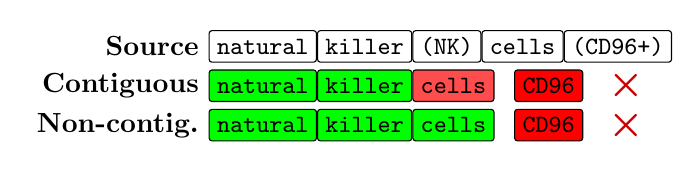
\begin{tikzpicture}[
  char/.style={
    draw, rounded corners=1pt,
    minimum height=4mm,
    inner xsep=1mm,  % horizontal padding inside variable-width boxes
    inner ysep=0pt,
    font=\ttfamily\small, align=center
  },
  idx/.style={font=\scriptsize, text=black!60},
  match/.style={dashed, thick, black!60}
]
\def\xgap{0mm} % gap between boxes

% --- Source ---
\node[anchor=east, font=\bfseries] at (0,0) {Source};

\foreach \c [count=\i] in {natural,killer,\symbol{40}NK\symbol{41},cells,\symbol{40}CD96+\symbol{41}} {
  \ifnum\i=1
    \node[char, anchor=west] (s\i) at (0,0) {\c};
  \else
    \node[char, right=\xgap of s\the\numexpr\i-1\relax] (s\i) {\c};
  \fi
}

% --- Contiguous ---
\node[anchor=east, font=\bfseries] at (0,-0.5) {Contiguous};

\foreach \c [count=\i] in {natural,killer,cells} {%
  % up to (and including) the space before "cells" is i<=15
  \ifnum\i<3
    \def\myfill{green}%
  \else
    \def\myfill{red!70}%
  \fi

  \ifnum\i=1
    \node[char, fill=\myfill, anchor=west] (t\i) at (0,-.5) {\c};
  \else
    \node[char, fill=\myfill, right=\xgap of t\the\numexpr\i-1\relax] (t\i) {\c};
  \fi
}

\node[anchor=west, font=\bfseries] (genelabel1) at (t3.east) {};

\foreach \c [count=\i] in {CD96} {
  \ifnum\i=1
    \node[char, anchor=west, fill=red] (g1\i) at (genelabel1.east) {\c};
  \else
    \node[char, right=\xgap of g1\the\numexpr\i-1\relax, fill=red] (g1\i) {\c};
  \fi
}
\node[anchor=west, font=\Large, text=red!80!black]
  at ([xshift=2mm]g11.east) {$\boldsymbol{\times}$};

% --- Non-contiguous ---
\node[anchor=east, font=\bfseries] at (0,-1) {Non-contig.};
\foreach \c [count=\i] in {natural,killer,cells} {
  \ifnum\i=1
    \node[char, anchor=west, fill=green] (t\i) at (0,-1) {\c};
  \else
    \node[char, right=\xgap of t\the\numexpr\i-1\relax, fill=green] (t\i) {\c};
  \fi
}

\node[anchor=west, font=\bfseries] (genelabel2) at (t3.east) {};

\foreach \c [count=\i] in {CD96} {
  \ifnum\i=1
    \node[char, anchor=west, fill=red] (g2\i) at (genelabel2.east) {\c};
  \else
    \node[char, right=\xgap of g2\the\numexpr\i-1\relax, fill=red] (g2\i) {\c};
  \fi
}
\node[anchor=west, font=\Large, text=red!80!black]
  at ([xshift=2mm]g21.east) {$\boldsymbol{\times}$};

\end{tikzpicture}
    
    % ---------------- CHAR-LEVEL ----------------
    \centerline{\textbf{Phrase alignment}}
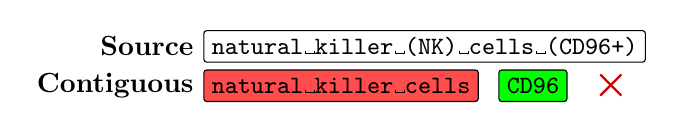
\begin{tikzpicture}[
  char/.style={
    draw, rounded corners=1pt,
    minimum height=4mm,
    inner xsep=1mm,  % horizontal padding inside variable-width boxes
    inner ysep=0pt,
    font=\ttfamily\small, align=center
  },
  idx/.style={font=\scriptsize, text=black!60},
  match/.style={dashed, thick, black!60}
]
\def\xgap{0mm} % gap between boxes

% --- Source ---
\node[anchor=east, font=\bfseries] at (0,0) {Source};

\foreach \c [count=\i] in {natural\textvisiblespace killer\textvisiblespace \symbol{40}NK\symbol{41}\textvisiblespace cells\textvisiblespace \symbol{40}CD96+\symbol{41}} {
  \ifnum\i=1
    \node[char, anchor=west] (s\i) at (0,0) {\c};
  \else
    \node[char, right=\xgap of s\the\numexpr\i-1\relax] (s\i) {\c};
  \fi
}

% --- Contiguous ---
\node[anchor=east, font=\bfseries] at (0,-0.5) {Contiguous};

\foreach \c [count=\i] in {natural\textvisiblespace killer\textvisiblespace cells} {%
  % up to (and including) the space before "cells" is i<=15
  \ifnum\i<1
    \def\myfill{red}%
  \else
    \def\myfill{red!70}%
  \fi

  \ifnum\i=1
    \node[char, fill=\myfill, anchor=west] (t\i) at (0,-.5) {\c};
  \else
    \node[char, fill=\myfill, right=\xgap of t\the\numexpr\i-1\relax] (t\i) {\c};
  \fi
}

\node[anchor=west, font=\bfseries] (genelabel1) at (t1.east) {};

\foreach \c [count=\i] in {CD96} {
  \ifnum\i=1
    \node[char, anchor=west, fill=green] (g1\i) at (genelabel1.east) {\c};
  \else
    \node[char, right=\xgap of g1\the\numexpr\i-1\relax, fill=red] (g1\i) {\c};
  \fi
}

\node[anchor=west, font=\Large, text=red!80!black]
  at ([xshift=2mm]g11.east) {$\boldsymbol{\times}$};
\end{tikzpicture}
  }
}

\caption{An example of common text-extraction and verification tasks using text from \citep{Hildreth2021}. LLMs correctly extract marker genes from a sentence, but exact and word-level alignment fail (red). The example cell-type and marker gene are found (green) only when aligned with non-contiguous alignment under subword or character tokenization.}
\label{fig:example}
\end{figure*}

One way to verify the existence of non-contiguous phrases is with LLM-as-a-judge \citep{gu2025surveyllmasajudge}. In this setting, language models are given a passage and extracted piece of text and are prompted to determine its existence. While sometimes effective, LLM-as-a-judge is mismatched to the task. Text is a concrete feature of a passage whereas LLM judgments are semantic and probabilistic distributions over a vocabulary (that includes text from the passage, as well as other text). Therefore, LLMs may approve paraphrases, or hallucinate, making them unsuitable for verifying the existence of text. We return to this comparison directly in Results, where a current model performing the alignment task itself refuses, misplaces, or miscopies evidence that exact alignment finds.

Practical issues with LLMs compound this problem. LLM inference is slow, expensive, and non-deterministic. For example, using \texttt{gpt-5.1} (\$1.25 per million input tokens, \$10 per million output tokens pricing as of late 2025), verifying a single 10-character string in a 1,000-character passage costs approximately \$0.001 and takes 1--2 seconds. Across 100,000 verifications, this amounts to tens to hundreds of dollars and tens of hours of compute for a check that string matching performs without a model call.

\begin{table*}[t!]
  \centering
  \caption{
  \textbf{The Berkeley Ordered Alignment of Text (\texttt{BOAT}) dataset} consists of multiple human-annotated text extractions derived from the \texttt{SQuAD} dataset. Each example includes a target text and a corresponding source text, where the target can be identified by direct string matching in the source. \texttt{BOAT} has two parts: a contiguous one, where the full target appears in the source, and a non-contiguous one, where part of the target is ablated and the target cannot be found contiguously. We report the average character (Char), whitespace-delimited word (WS), and subword token (Tok) lengths of both source and target texts. WS corresponds to word-level, and Tok to subword tokenization. Alignment counts ($N_{\text{0-align}}$, $\mu_{\text{align}}$, $\mu_{\text{match}}$) are computed with \texttt{taln} under punctuation-aware tokenization; $\mu_{\text{align}}$ counts order-preserving alignments and $\mu_{\text{match}}$ counts unique source matches. The 196 targets that remain contiguous after token deletion are excluded from the non-contiguous row. We also report the same statistics for the \texttt{BIO-BOAT} dataset.
  }
  \begin{tabular}{llrrrrrrrr}
  \toprule
  \textbf{\texttt{BOAT}} & $\mathbf{N}$ & $\mathbf{N_{\text{0-align}}}$ (\%) & $\mathbf{\mu_{\text{align}}}$ & $\mathbf{\mu_{\text{match}}}$ & \textbf{Text} & \textbf{Chars} & \textbf{WS} & \textbf{Tok} \\ 
  \midrule
  
  \multirow{2}{*}{}
   Contiguous & 35{,}080 & 47 (0.1) & 8.9 & 2.5 & source & 764 & 121 & 158\\
              &          &     &     &     & target & 38  & 6 & 8 \\
  \midrule
  
  \multirow{2}{*}{}
    Non-contiguous & 34{,}884 & 45 (0.1) & 8.7 & 2.6 & source & 764 & 121 & 158\\
                   &          &           &     &     & target & 33  & 5   & 7 \\
  \midrule
  \multirow{2}{*}{}
    Contiguous (\texttt{BIO}) & 5{,}316 & 126 (2.4) & 28.1 & 2.1 & source & 607 & 91 & 132\\
                              &         &           &      &     & target & 97  & 14 & 20\\
  \midrule
  \multirow{2}{*}{}
    Non-contiguous (\texttt{BIO}) & 5{,}316 & 126 (2.4) & 28.4 & 2.1 & source & 607 & 91 & 132\\
                                  &         &           &      &     & target & 90  & 13 & 18\\
  \bottomrule
  \end{tabular}
  \label{tab:BOAT}
  \end{table*}

But as we saw, exact string matching is insufficient. More complex methods---that split the phrase and align parts of it---offer an improvement. By splitting the text into units (also known as tokens) and aligning each independently, rather than matching consecutively occurring characters, these methods can align non-contiguous text. Because tokens only need to appear in the same order, non-contiguous matches become possible. Removing the contiguity constraint allows alignment to skip irrelevant parts of a sentence.

Tokens can, in principle, be any unit of text---from individual characters to full words or even multi-word expressions---but token size introduces a fundamental tradeoff \citep{whittington2024tokenisationnpcomplete}. Small tokens (e.g. characters) offer maximal flexibility. Every character can be aligned independently, allowing methods to recover highly fragmented phrases (Figure~\ref{fig:example}). But this flexibility is computationally expensive. If a phrase has $k$ characters and the source has $n$ characters (all the same), aligning at the character level can produce up to $\binom{n}{k} \approx \frac{n^k}{k!}$ possible non-contiguous matches. For example, aligning a 10-character target (e.g. \texttt{AAAAAAAAAA} to a 1,000 character (\texttt{A...A}) source produces roughly $10^{23}$ possible alignments, compared to only $n - k + 1 = 991$ matches for simple contiguous search. Conversely, very large tokens (e.g. whole sentences) reduce the search space by merging punctuation, symbols, acronyms, or alphanumeric identifiers in ways that may hide LLM-extracted phrases. Thus, token size directly determines what alignments are findable and computationally tractable.

A common tokenization method is word-level: text is split on the spaces between characters and tokens are whole words. But word-level tokenization breaks down in scientific text. As shown in Figure~\ref{fig:example}, if an LLM extracts the gene name ``\texttt{CD96}'' from the phrase ``\texttt{natural killer (NK) cells (CD96+)}'', word-level alignment fails because that tokenization merges the gene name with parentheses, and a plus sign. This situation is quite common. In biological text, gene names often contain characters like parentheses, plus signs, and mixed alphanumeric formatting that are inconsistently attached to genes, causing word-level methods to miss alignments.

In this work, we study how tokenization and alignment strategy affect the recovery of missing alignments resulting from non-contiguous phrases. This work focuses on explicitly extracted text instead of implicitly (semantically) extracted text, where the text is inferred from the context. We introduce two benchmark datasets, formalize text alignment to motivate a practical alignment method, and evaluate the impact of tokenization with this method. We then evaluate rules for selecting one source location among the enumerated alignments, and compare against an LLM performing the same alignment task. Based on these benchmarks, we release an open-source tool, called \texttt{taln}, for deterministic non-contiguous text alignment with source offsets.

\section{Results}
We constructed two benchmark datasets: \texttt{BOAT}, derived from \texttt{SQuAD} \citep{rajpurkar2016squad100000questionsmachine, rajpurkar2018knowdontknowunanswerable}, and \texttt{BIO-BOAT}, a biomedical extension built from 51 bioRxiv preprints (Table~\ref{tab:BOAT}). Using these datasets, and a formalization of alignment methods, we show that ordered alignment recovers non-contiguous phrases and that alignment accuracy is determined largely by how the text is tokenized. We then evaluate rules for selecting one source location among the enumerated alignments and compare against an LLM performing the same alignment task.

\subsection{Dataset design}
\texttt{BOAT} consists of 35{,}080 source–target pairs derived from \texttt{SQuAD}, where each target aligns contiguously in its source passage. Sources average 764 characters (121 whitespace tokens; 158 subword tokens), and targets average 38 characters (Table~\ref{tab:BOAT}). To evaluate non-contiguous alignment, we constructed a variant in which one interior token is removed from each target, ensuring that the resulting phrase can no longer be found by exact contiguous alignment. This variant is not a full simulation of errors in LLM-extraction workflows where extracted phrases fragmented into multiple non-contiguous tokens, but it is a useful proxy to test the sensitivity of alignment methods to non-contiguous phrases.

To test whether alignment behavior generalizes beyond general-domain text, we constructed \texttt{BIO-BOAT}, containing 5{,}316 source–target pairs extracted from 51 bioRxiv preprints, with both contiguous and non-contiguous variants (Methods) \citep{van_Vliet_2022,Cobo_L_pez_2023,Meyer_2023,Zimyanin_2023,Singer_2024,Shen_2024,Frolov_2024,Ryan_2024,Pfalzgraf_2024,Onishi_2024,Wondim_2024,Crnkovic_2024,Kallenborn_2024,Peroutka_Bigus_2024,Azim_2024,Bhalla_2024,Jones_2024,Fei_2024,Combredet_2024,Simmonds_2025,Adhinarta_2025,Elangovan_2025,Tang_2025,Maya_Miles_2025,Samame_Caramutti_2025,Nguyen_2025,Terstege_2025,Chen_2025_biorxiv,Li_2025,Kattner_2025,Shruti_2025,Vel_zquez_2025,Rull_2025,D_lker_2025,Keikhosravi_2025,Agazzi_2025,Choltus_2025,Maestro_2025,Widney_2025,Smith_2025,Mar_n_2025,Dadonaite_2025,Green_2025,S_lzen_2025,Pearce_2025,Biller_2025,Laub_2025,Johnson_2025,Na_2025,Tozzi_2025}. Biomedical text introduces denser punctuation, symbols, and alphanumeric identifiers, making it a stringent test for alignment methods and tokenizers (which are often built from general-domain texts.)

\subsection{Alignment algorithms}
Many alignment methods exist for verifying extracted text, from exact string matching to algorithms that allow gaps or reorderings. To compare them, we formalized alignment as a map from target token positions to source token positions (Supplementary Note).

Under this formalization, alignment methods form a hierarchy defined by the constraints they impose on this map. Contiguous alignment requires adjacent tokens to match. Ordered alignment drops adjacency but retains order. Permutation alignment drops order but requires a one-to-one correspondence. General rearrangement imposes no constraints. Each relaxation admits more valid alignments, but the number of possible alignments grows rapidly, from linear (contiguous) to factorial (permutation) to exponential (rearrangement).

Ordered alignment sits at a practical point in this hierarchy: it recovers non-contiguous phrases while keeping the number of alignments manageable. In practice, relaxing constraints beyond ordered alignment produces spurious alignments, making permutation and rearrangement impractical. We therefore focus our study on ordered alignment and implement it in a tool called \texttt{taln}, short for \textbf{T}oken \textbf{Al}igner. \texttt{taln} is a Python library and command-line tool that returns all order-preserving alignments between a target and source. \texttt{taln} is tokenizer-agnostic and supports various tokenization strategies. 


\begin{figure*}[ht!]
    \centering
    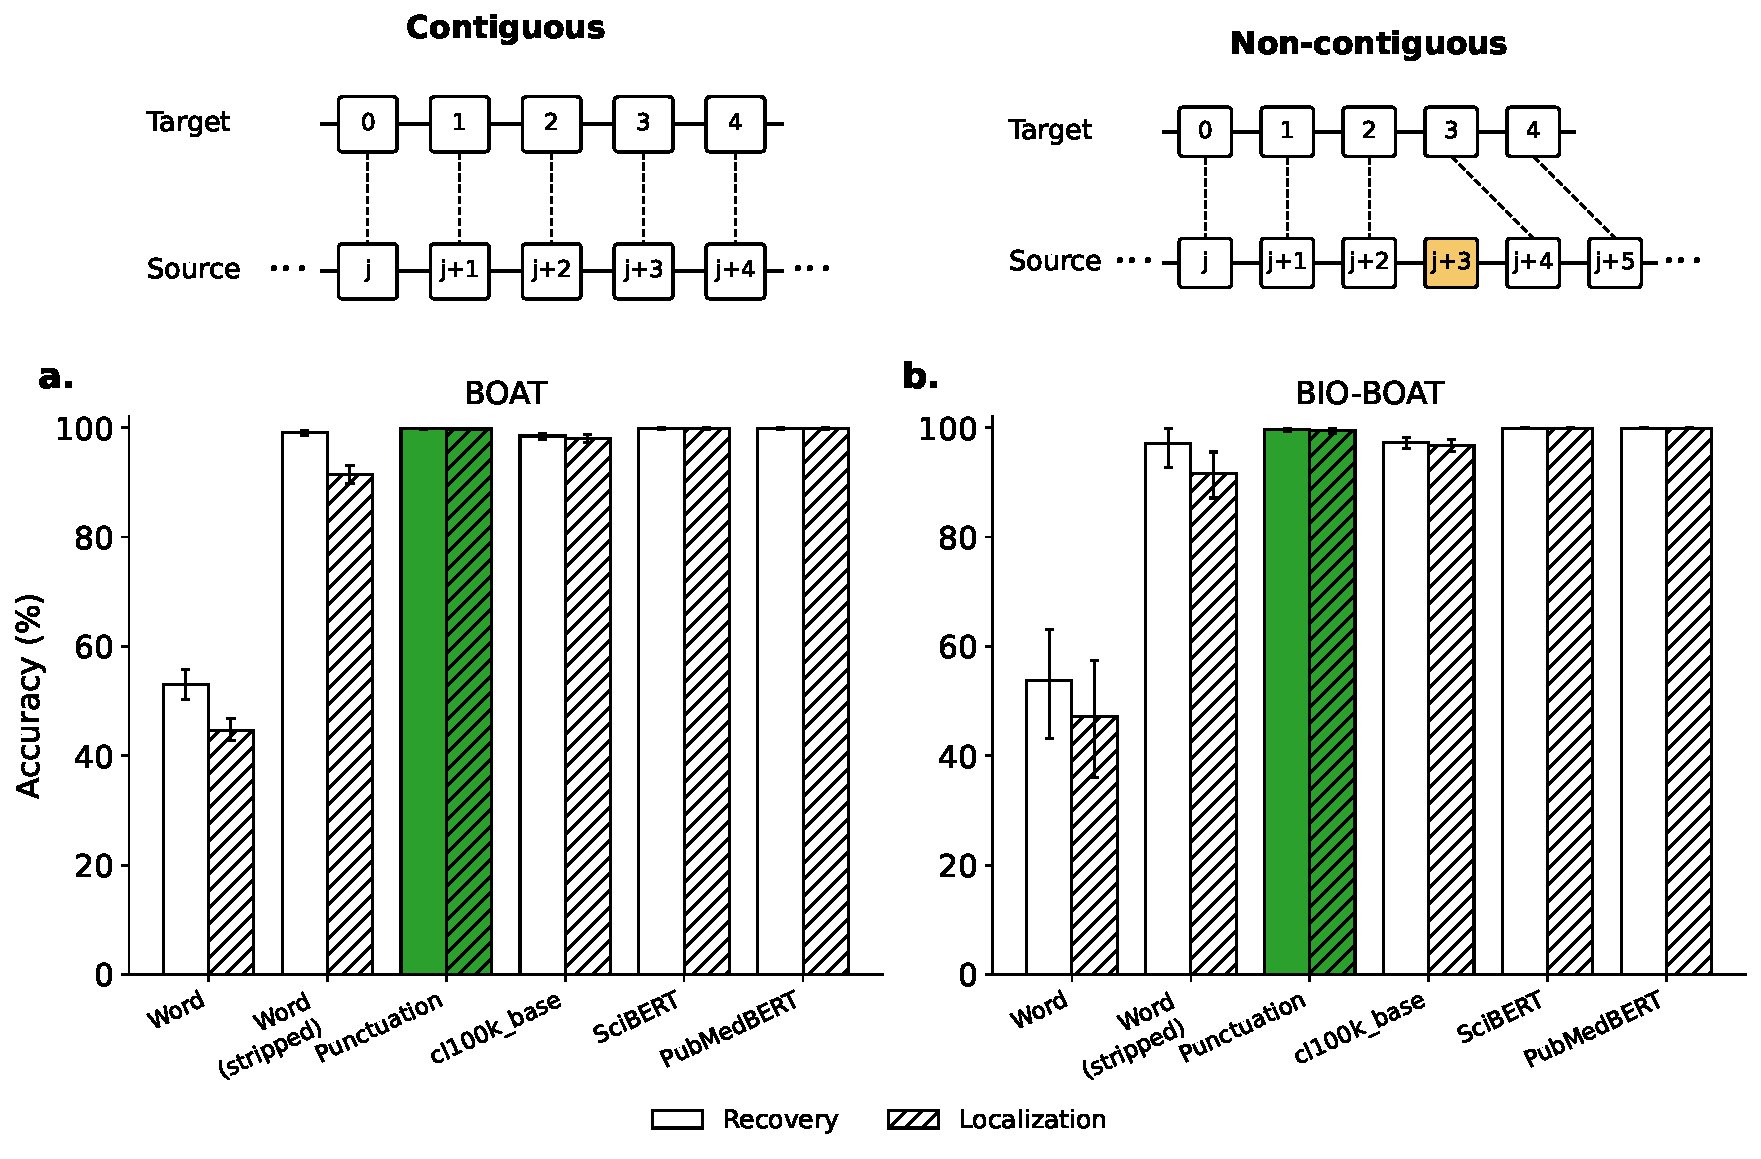
\includegraphics[width=0.95\linewidth]{../../shared/figures/tokenizer_comparison.pdf}
    \caption{\textbf{Tokenization determines non-contiguous alignment accuracy.} Top: ordered alignment maps target tokens to source tokens in order; a non-contiguous phrase skips source tokens (orange). \textbf{a.} Recovery (solid) and localization (hatched) for \texttt{taln} on held-out one-gap \texttt{BOAT} targets (n=4,284) under six tokenizers, with document-clustered 95\% confidence intervals. \textbf{b.} The same for \texttt{BIO-BOAT} (n=1,259). Contiguous recovery is within 0.1 percentage points of one-gap recovery for every tokenizer and is identical on \texttt{BIO-BOAT}.}
    \label{fig:tokenizer}
\end{figure*}

\subsection{Text Tokenization}
Having selected an alignment algorithm, we next asked how tokenization affects alignment accuracy. We compared exact string matching against ordered alignment under six tokenizers: word-level (whitespace), word-level with punctuation stripped from token boundaries, a punctuation-aware tokenizer that keeps each punctuation mark as its own token, subword tokenization using the \texttt{cl100k\_base} tokenizer, and two biomedical subword tokenizers (SciBERT and PubMedBERT) (Methods). We benchmarked \texttt{taln}, longest common subsequence (LCS), exact semi-global alignment, and Python's \texttt{difflib.SequenceMatcher} on held-out contiguous and non-contiguous variants of \texttt{BOAT} and \texttt{BIO-BOAT}. Alignment accuracy depended on the tokenizer far more than on the alignment method.

\subsubsection{Contiguous text}
On held-out contiguous phrases from \texttt{BOAT}, exact string matching recovered all targets, as expected. In contrast, under word-level tokenization, ordered alignment recovered only 2,278 of 4,313 targets (52.8\%) despite every phrase being fully contiguous (Figure~\ref{fig:tokenizer}a).

These failures arose from punctuation attached to neighboring words. For example, quotation marks and commas are often omitted from the beginning or end of \texttt{SQuAD} answers (e.g. \texttt{a lawless place'' or ``a place under no jurisdiction}) even when present in the passage (\texttt{...of ``a lawless place'' or ``a place under no jurisdiction''...}). When split by whitespace, the missing adjacent quotes prevent the affected word tokens from matching, causing otherwise contiguous phrases to be missed.

To test this mechanism directly, we kept whitespace tokenization but stripped punctuation from the outer boundaries of each token. This single change raised recovery to 4,271 of 4,313 targets (99.0\%). A punctuation-aware tokenizer that keeps each punctuation mark as its own token recovered 4,303 of 4,313 (99.8\%), and subword tokenization with \texttt{cl100k\_base} recovered 4,247 of 4,313 (98.5\%). The difference between word-level and subword tokenization is a token-boundary effect: subword tokenizers separate punctuation from words, and a word-level tokenizer that handles punctuation achieves the same recovery.

\subsubsection{Non-contiguous text}
To evaluate alignment on non-contiguous phrases, we used the held-out one-gap \texttt{BOAT} dataset (n=4,284). In this setting, exact string matching failed entirely (0\%). Under word-level tokenization, ordered alignment recovered 2,270 of 4,284 targets (52.99\%). Punctuation-aware tokenization recovered 4,275 of 4,284 (99.79\%), an improvement of 46.80 percentage points (document-clustered 95\% CI, 44.11 to 49.33), and subword tokenization with \texttt{cl100k\_base} recovered 4,219 of 4,284 (98.48\%). Localization tracked recovery for every tokenizer except boundary-stripped word tokenization, which recovered 99.07\% of targets but localized only 91.41\%: stripping punctuation finds the tokens, and the reported match boundaries then exclude the attached punctuation that the correct location includes.

The recovery rates match the contiguous setting almost exactly. Deleting an interior token leaves the remaining tokens in source order, so alignment is dependent on variation in tokenization. Allowing gaps is necessary to align non-contiguous phrases, but which phrases can be aligned is decided by the token boundaries.

Under the same tokenization strategy, \texttt{taln}, LCS, and semi-global alignment always agreed on whether a target could be aligned. \texttt{difflib.SequenceMatcher}, a matching-block heuristic, missed some valid ordered alignments and never recovered an alignment the exact methods missed. \texttt{taln} differs from the other methods by reporting every order-preserving alignment, along with the positions in the source that support each one.

\subsubsection{Generalization to biomedical text}
To test whether these results generalize to biomedical text, we repeated the evaluation on held-out \texttt{BIO-BOAT} (n=1,259). The same pattern holds (Figure~\ref{fig:tokenizer}b): word-level tokenization recovered 53.85\% of one-gap targets, punctuation-aware tokenization recovered 99.68\%, an improvement of 45.83 percentage points (95\% CI, 36.64 to 56.42), and subword tokenization with \texttt{cl100k\_base} recovered 97.22\%. Contiguous and one-gap recovery were identical under every tokenizer. The same four records failed in both conditions. All four are text-conversion artifacts in which a word is fused with adjacent text: three carry a trailing citation number (e.g. \texttt{properties38,39}) and one is joined to a section header (\texttt{AbstractPreeclampsia}).

We then asked whether biomedical tokenizers improve on this. SciBERT and PubMedBERT recovered 1,258 of 1,259 held-out one-gap targets (99.92\%), compared with 1,255 of 1,259 (99.68\%) for punctuation-aware tokenization---a difference of three targets (0.24 percentage points; 95\% CI, 0.00 to 0.54). The three recovered targets are the citation-number fusions: subword vocabularies split at the letter--digit boundary (\texttt{properties38} into \texttt{properties} and \texttt{38}), which a word-level tokenizer keeps as one token. The fused section header was recovered by no tokenizer. A punctuation-aware tokenizer removes most alignment failures, and the additional benefit of biomedical tokenizers is minimal in this sample.

In practice, punctuation-aware and subword tokenization both reach near-complete recovery, and subword tokenization has a structural appeal for LLM-extraction workflows: the extracted text is verified over the same kind of objects the model generated.

\begin{figure*}[ht!]
    \centering
    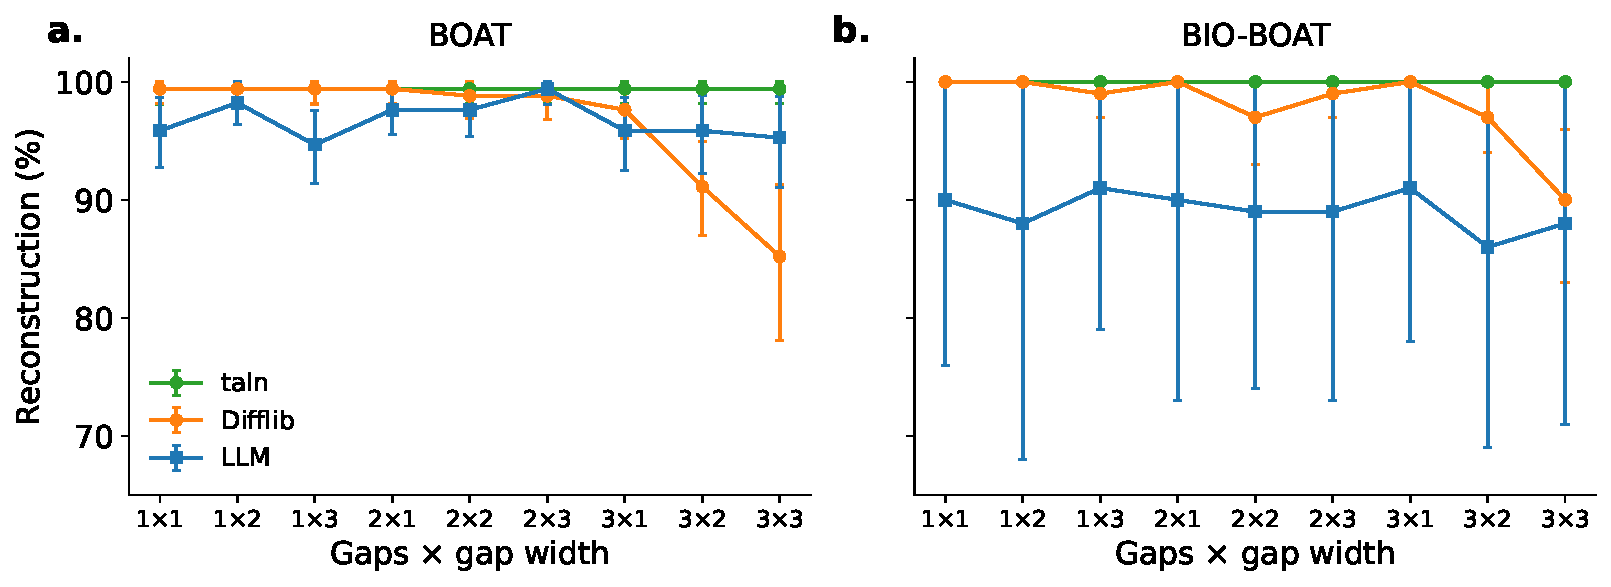
\includegraphics[width=0.95\linewidth]{../../shared/figures/multigap_llm.pdf}
    \caption{\textbf{Exact ordered alignment is invariant to fragmentation.} Reconstruction by gap count and gap width for \texttt{taln}, \texttt{difflib}, and an LLM given the same alignment task, with document-clustered 95\% confidence intervals. \textbf{a.} \texttt{BOAT} (169 records from 27 held-out documents). \textbf{b.} \texttt{BIO-BOAT} (100 records from 10 held-out documents). All three methods were evaluated on the identical sample, drawn at up to 10 records per document so that no document dominates. Exact string matching recovered no variant in any condition and is not shown.}
    \label{fig:multigap}
\end{figure*}

\subsection{Multi-gap alignment}
The one-gap construction tests a single interior deletion. Extracted phrases can also drop several separated pieces of a source sentence, so we next asked whether alignment recovery changes as one gap becomes several. Starting from 5,863 source--target pairs across 300 documents, we deleted one to three interior blocks of one to three tokens each, producing 58,630 variants under a full factorial of gap count and gap width (Methods). Each shortened target remains an ordered subsequence of its unchanged source, so this is a controlled stress test of alignment behavior.

On the 8,720 held-out variants, ordered alignment under punctuation-aware tokenization was unaffected by the number and width of gaps (Figure~\ref{fig:multigap}). At the most severe condition (three gaps of width three), \texttt{taln} recovered 334 of 337 \texttt{BOAT} records (99.1\%) and 535 of 535 \texttt{BIO-BOAT} records (100.0\%), identical to its recovery of the unmodified contiguous controls. Exact string matching recovered no non-contiguous variant, and LCS agreed with \texttt{taln} on every variant.

\texttt{difflib.SequenceMatcher} degraded as gaps accumulated. At three gaps of width three it recovered 292 of 337 \texttt{BOAT} records (86.6\%; 95\% CI, 82.1 to 89.8) and 496 of 535 \texttt{BIO-BOAT} records (92.7\%; 95\% CI, 89.0 to 95.4). Across all held-out conditions there were 373 disagreements between \texttt{difflib} and the exact methods, every one favoring the exact methods. We audited all 373 and found that in each case a complete ordered alignment exists, but \texttt{difflib}'s greedy matching-block heuristic committed to an early block that made the rest of the target unmatchable. Fragmented phrases therefore require an exact ordered method since a heuristic can lose valid alignments.

\subsection{Alignment enumeration}
Unlike LCS and \texttt{difflib}, \texttt{taln} enumerates all valid alignments rather than returning a single match. This matters when extracted phrases appear multiple times in a passage---common in scientific text where repeated entities (gene names, conditions, acronyms) may indicate importance \citep{swayamdipta2018multimention, zhang2023howmanyanswers, moon2023extractive, wang2024mesaqa}.

On the 13,351 held-out non-contiguous targets from the one-gap and multi-gap benchmarks, most targets had a single supporting location (Figure~\ref{fig:selection}a). The median number of unique source matches was 1, and 5,735 targets (43.0\%) had more than one (95th percentile 8, maximum 176). Raw alignment counts run higher (95th percentile 22, maximum 29,468) because repeated tokens multiply the distinct token-level paths through the same stretch of text; collapsing alignments to unique source matches removes most of this multiplicity. Tokenization adds its own multiplicity. Under subword tokenization, a gene name such as \texttt{VEGF-A165b} decomposes into five tokens, each of which may match at several positions.

\begin{figure*}[ht!]
    \centering
    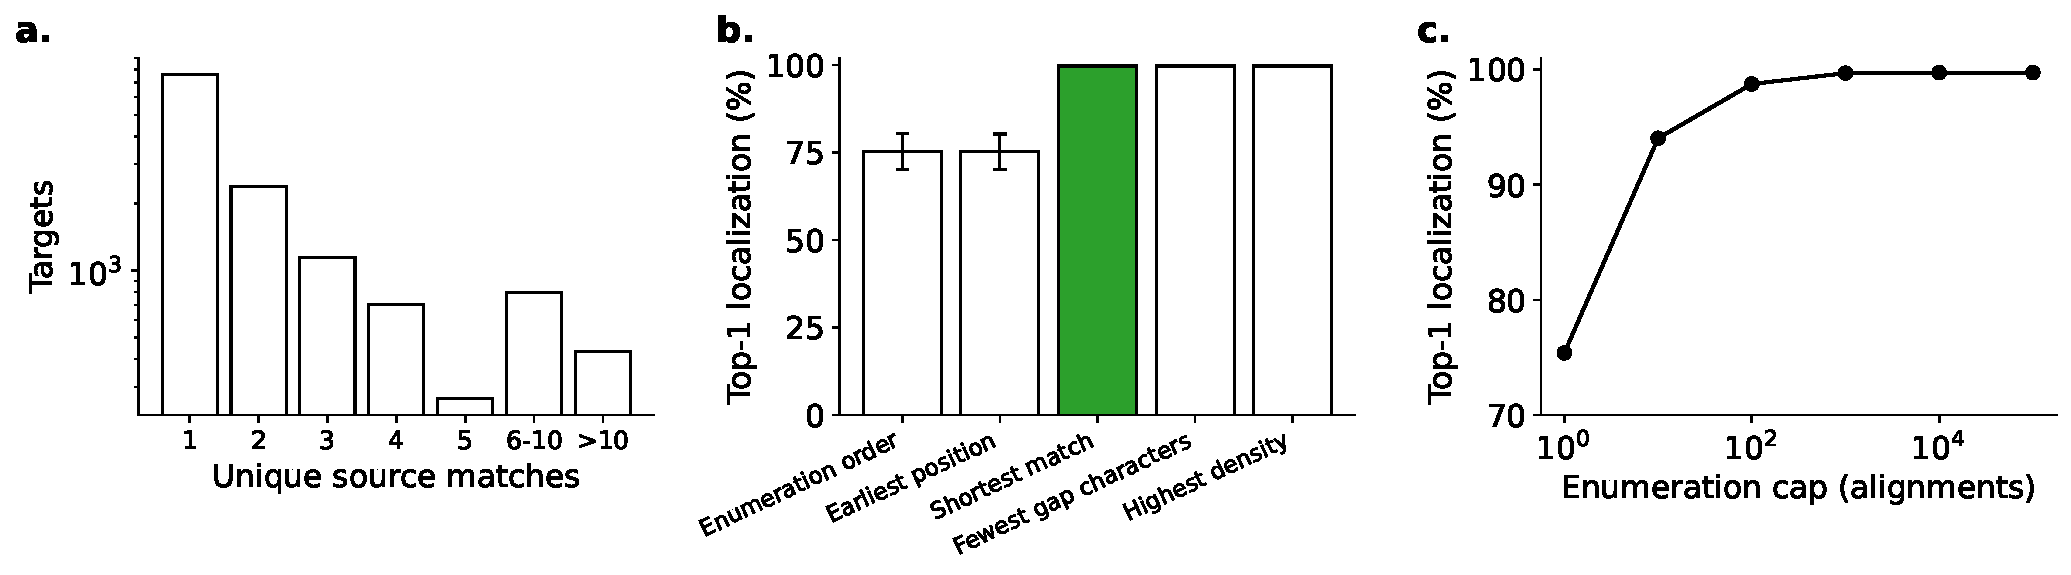
\includegraphics[width=\linewidth]{../../shared/figures/selection_assessment.pdf}
    \caption{\textbf{Selecting one source location from enumerated alignments.} \textbf{a.} Number of unique source matches per fully supported held-out non-contiguous target (n=13,351, punctuation-aware tokenization); 5,735 targets (43.0\%) have more than one. \textbf{b.} Top-1 localization for five parameter-free selection rules with document-clustered 95\% CIs; the selected rule (shortest match, green) identifies a correct location first for 99.74\% of targets. Shortest match, fewest gap characters, and highest density make identical selections. \textbf{c.} Top-1 localization of the shortest-match rule as a function of the enumeration cap; complete enumeration is required to reach full selection accuracy.}
    \label{fig:selection}
\end{figure*}

The tradeoff for enumeration returning every supporting location is that an alignment workflow must still select among them. We evaluated five parameter-free selection rules: enumeration order, earliest position, shortest source match, fewest gap characters, and highest matched-token density (Methods). Shortest source match, a selection rule that prefers the candidate covering the fewest source characters, identified a correct location first for 13,316 of 13,351 held-out targets (99.74\%; 95\% CI, 99.53 to 99.87), and within its top five for 99.90\% (Figure~\ref{fig:selection}b). Taking alignments in enumeration order identified a correct location first for 75.40\%. The three rules that prefer compact matches (shortest match, fewest gap characters, highest density) made identical selections on every target and are one effective rule.

Selection accuracy depends on complete enumeration (Figure~\ref{fig:selection}c). Capping enumeration at one alignment reduces the shortest-match rule to enumeration order (75.40\%); caps of 100 and 1,000 recover 98.75\% and 99.69\%. \texttt{taln} therefore enumerates completely by default and reports an explicit truncation status when a user-set cap is reached. Selection also has a floor. In 75 targets (0.56\%), identical text appears at both a correct and an incorrect location, and no rule that reads only the text can distinguish them. Choosing among lexically identical occurrences requires context beyond the alignment itself.

\subsection{LLM-based alignment}
The extracted text in these workflows is produced by an LLM, so a natural question is whether the same model can also locate its evidence, replacing an alignment algorithm. We asked \texttt{claude-sonnet-4-5} to perform the identical lexical task: given the source and the submitted text, return the verbatim source excerpts that contain the submitted words in order. Returned excerpts were located in the source by exact search---the model never reports character positions---and scored with the same metrics as the alignment methods, on a document-sampled subset of the held-out benchmarks (2,153 targets spanning contiguous, one-gap, and three-gap conditions). The prompt was developed on separate documents and frozen before evaluation (Methods). Every sampled target has complete lexical support by construction, so this comparison measures whether the model can produce and locate the evidence, not whether it can reject unsupported text.

The model produced complete verbatim evidence for 2,083 of 2,153 targets (96.75\%) and a correct source location for 96.01\%. On the same targets, \texttt{taln} reconstructed 99.91\% and localized 99.72\%. On general-domain text the model was close to exact alignment (99.72\% contiguous, 98.87\% one-gap). On biomedical text it dropped to 94.97\% (contiguous), 95.99\% (one-gap), and 92.70\% (three gaps), and all of the difference beyond alignment error came from model-specific failure modes.

Fragmentation did not drive these failures (Figure~\ref{fig:multigap}). Across the nine gap conditions the model recovered 94.7\% to 99.4\% of \texttt{BOAT} targets and 86.0\% to 91.0\% of \texttt{BIO-BOAT} targets, with no trend as gaps accumulated. Its failures arise from the passage and the model. \texttt{difflib} shows the opposite pattern. Its recovery falls as gaps accumulate, reaching 85.2\% on \texttt{BOAT} at three gaps of width three, where the model recovered 95.3\% and \texttt{taln} recovered 99.4\%.

Those failure modes do not exist for a deterministic method. The model refused to process 46 biomedical passages, returning no output; the same passages refused again on a second attempt. It returned evidence at a wrong location for 16 targets, declared 8 supported targets unsupported, returned unparseable replies for 7, and copied excerpts that were not verbatim in the source for 3. In one representative case the model identified the correct excerpt in its reasoning and then returned the submitted text, rather than the source text, as its excerpt. Exact lexical alignment does not need to be delegated to a generative model, and delegating it introduces refusal, copying, and format errors that exact enumeration cannot make.

\subsection{Natural marker records}
The benchmarks above construct non-contiguous targets by simulated deletion. To test alignment on labels that arise naturally, we used a human-curated marker corpus built from seven single-cell studies, called \texttt{llmarkers}. This corpus contains cell-type and marker-gene labels copied from a manuscript passage. We aligned each label against its recorded passage: 877 records with prose evidence, giving 512 unique label--passage pairs (140 cell-type, 372 marker-gene).

Alignment of these labels reproduced the tokenizer results from the constructed benchmarks. Word-level tokenization recovered 216 of 512 pairs (42.2\%). Punctuation-aware tokenization recovered 506 (98.8\%), and \texttt{cl100k\_base} recovered 511 (99.8\%). Subword tokenization beats out the punctuation-aware tokenizer, and the mechanism is visible in the failures. Often, biomedical prose contains PDF-to-text conversion artifacts like citation numbers directly attached to words, as in \texttt{human regulatory T cells17}. A punctuation-aware tokenizer keeps \texttt{cells17} as one token and the label's \texttt{cells} cannot match; a subword tokenizer splits at the letter--digit boundary and recovers it. Citation fusion accounts for four of the six punctuation-aware failures.

Individual records show where alignment succeeds and where it stops. The label \texttt{Iris stroma Schwann cells} is non-contiguous in its passage (``Iris stroma is also populated by Schwann cells...''): exact matching fails and ordered alignment recovers it. The label \texttt{GAS2} was curated from the compact notation \texttt{GAS1/2}, which subword alignment recovers and word-level alignment cannot. One label was recovered by no tokenizer: \texttt{WIF1-high fibroblast}, curated in the singular where the passage writes \texttt{fibroblasts}. On natural marker records, ordered alignment under a punctuation- or subword-aware tokenizer recovers nearly every label, and the failures that remain are differences of meaning rather than of matching.

\balance

\section{Discussion}
LLMs are powerful tools for data mining. They can ingest massive amounts of text and rapidly synthesize, extract, and return specific pieces of information. But unlike other data-mining tasks, such as summarization, text extraction has a strict constraint on the generated text: the output must already exist in the input. Humans can often verify that this constraint is not violated, but doing so at scale becomes prohibitive. This is where text-alignment algorithms can assist human evaluators by providing automated, verifiable checks. Our results show that this constraint can be checked deterministically with token-based alignment, and that delegating the check to an LLM reintroduces the kinds of errors the check exists to catch.

Alignment algorithms are well suited to this verification task, but traditional text alignment algorithms and tokenization strategies struggle with scientific text---despite their long history and development in disparate fields \citep{hirschberg1975lcs, KnuthMorrisPratt1977, Melsted2021, sennrich2016neuralmachinetranslationrare, Sullivan2025}. Extracted phrases are often interrupted by symbols, qualifiers, or parenthetical statements. Exact phrase matching therefore misses many valid alignments. Alignment methods that allow gaps or skips between aligned segments offer a practical solution, but they introduce a new question: what constitutes a meaningful ``part'' of a phrase?

This work shows that the answer is decided by tokenization. Word-level tokenization treats each whitespace-delimited word as an alignable part of a sentence, so a quotation mark or comma attached to a word changes the accuracy of alignment. Subword tokenization splits punctuation and word pieces into separate parts, and the same match, which would otherwise fail, succeeds. The difference then largely arises from token boundaries which are influenced by the corpus used to create the tokenizer. Subword tokenization is a natural choice for LLM-extraction workflows because the extracted text is aligned over the same kind of sentence parts the language model generated. In this work, exact ordered methods agreed on which targets could be aligned under every punctuation-aware tokenizer. The benefit that \texttt{taln} provides is enumerating every alignment with its source positions.

However, enumerating many valid alignments introduces a new challenge of selecting the most meaningful one. As alignment recovery improves, selecting the correct alignment becomes the limiting factor. Our selection analysis shows that a simple rule---prefer the shortest source match---identifies a correct location first for 99.74\% of held-out non-contiguous targets. This rule depends on complete enumeration. When limited to returning only a single alignment, its accuracy falls to that of enumeration order. Selection also has a lexical bound that only semantic judgment can overcome. When identical text appears at several locations, choosing among them requires context beyond the alignment. Methods for verifying the existence of LLM-extracted phrases with semantic or implicit matching (instead of explicit matching) are a promising direction for improving this bound, but are outside the scope of this work.

These results also hold in biomedical text, where tokens tend to be more duplicative and where selection becomes increasingly important. Alignment multiplicity is higher in biomedical text because repeated gene names and identifiers produce more valid locations per target, which raises the burden on selection. Domain-specific tokenization improves recovery at the margin; alignment selection remains a separate step.

The task of verifying extracted text is closely related to biological sequence mapping in principle, but the matching criterion differs (Supplementary Note). Read mappers and tools such as BLAST use seed-and-extend and scoring heuristics to find high-scoring approximate matches in large references \citep{Altschul_1990}. For text matching, the goal is stricter: verify whether an extracted text string is explicitly supported by source tokens and identify its position. Approximate sequence-alignment ideas are therefore relevant for indexing, ranking, and scaling, but mismatch-tolerant biological mapping is not a drop-in replacement for exact text alignment.

These results show that alignment algorithms and tokenization matter for verifying LLM-extracted text, and how methods from computational biology and linguistics can be combined to develop useful verification tools. This matters because LLM-based extraction is increasingly used to structure information from scientific, medical, and other data-intensive texts, where unverified outputs can propagate errors and undermine trust. By providing deterministic and transparent token-based alignment, \texttt{taln} supports extraction workflows in which passages can be extracted contiguously from large documents, and relevant---possibly non-contiguous---text can then be aligned back to those passages before downstream use.

\clearpage
\newpage
\onecolumn
\appendix

\section{Methods}
\subsection{\texttt{BOAT} Building}
We derived \texttt{BOAT} from the Stanford Question Answering Dataset (\texttt{SQuAD}) v2.0. Each \texttt{SQuAD} example provides a passage (source), an answer string (target), and an answer start index (\texttt{answer\_start}) locating the target as a contiguous character sequence in the source.

We first flattened \texttt{SQuAD} into records with fields \texttt{source}, \texttt{target}, and \texttt{idx\_start} (plus metadata such as title and question identifiers). We retained records where an exact contiguous string match occurs:  $\texttt{source[idx\_start:idx\_start+len(target)]} = \texttt{target}.$ We then deduplicate on \texttt{(source, target, idx\_start)}.

To make character indices consistent with subword tokenization, we applied a ``shift'' normalization: if the character immediately preceding \texttt{idx\_start} is a space, we prepend a space to the target and decrement \texttt{idx\_start} by one. This ensures that leading whitespace, when present in the source, is part of the target phrase; a feature that is often seen in substring tokenization vocabularies. Note this does not affect whitespace tokenization since the space is prepended to the string.

Because identical \texttt{(source, target)} pairs can occur with multiple valid start indices (e.g., repeated mentions in a passage), we grouped by \texttt{(source, target)} and stored \texttt{idx\_start} as a set of start positions. In downstream analyses we restricted to multi-word targets to focus on phrases where ablating an interior token introduces a meaningful non-contiguity.

We constructed two \texttt{BOAT} variants: Contiguous \texttt{BOAT} and Non-contiguous \texttt{BOAT}. Contiguous \texttt{BOAT} consists of the original \texttt{(source, target)} pairs and their \texttt{idx\_start} sets. Non-contiguous \texttt{BOAT} was constructed by removing the central interior word of each target, so the remaining words cannot be found by contiguous matching.

\subsubsection{\texttt{BIO-BOAT} Building}
We downloaded 51 papers from the bioRxiv AWS bucket \texttt{s3://biorxiv-src-monthly/Current\_content/}, dated January 2025 and licensed under CC BY 4.0. We converted the manuscript XML to Markdown and ran \texttt{taln extract}, which prompts an LLM (\texttt{claude-sonnet-4-20250514}) to return source–target pairs from each paper, and retained only pairs whose target occurs verbatim and contiguously in its source. The extraction step determines which strings enter the benchmark; it plays no role in evaluation, which measures whether alignment methods recover strings already known to be present. We then generated non-contiguous \texttt{BIO-BOAT} in the same manner as \texttt{BOAT} described above.

\subsection{Multi-gap construction}
We treated maximal non-whitespace runs of the target as chunks and kept targets with at least 13 chunks, so that every target supports every condition. For each combination of gap count (1 to 3) and gap width (1 to 3 chunks), we deleted the chosen blocks and spread the retained chunks as evenly as possible around them, assigning any remainder left to right. The unmodified target serves as a contiguous control. A shortened target that still occurs as an exact substring of the source was labeled a control and excluded from non-contiguous summaries. Enumeration was capped at 100,000 alignments per target, and the cap status was recorded. No held-out target reached the cap.

\subsection{Natural marker records}
The natural benchmark uses a marker corpus that we hand-curated from seven single-cell studies, called \texttt{llmarkers} (\href{https://github.com/sbooeshaghi/llmarkers}{https://github.com/sbooeshaghi/llmarkers}). For each reported marker association, we recorded the cell-type label, the marker-gene label, and the manuscript passage reporting it, copying the labels verbatim from the passage. We used the 877 records whose evidence is manuscript prose; records curated from figures carry no passage text and were excluded. Each record contributes two label--passage pairs, one for each label. Labels carry leading or trailing whitespace from manual selection, which we strip, and repeated pairs are collapsed to 512 unique pairs for the primary analysis. The corpus asserts only real marker associations. It contains no curator-marked negatives, so it measures recovery and supports no false-acceptance claim. The curation predates \texttt{taln} and was performed without exposure to any alignment output.

\subsection{Text Tokenization}
We evaluated six tokenizers. Word-level tokenization splits on whitespace; each token is a maximal non-whitespace run. Boundary-stripped word tokenization additionally removes punctuation from the outer edges of each word token. Punctuation-aware tokenization keeps each run of letters or digits as a token and each punctuation mark as its own token. Subword tokenization uses the OpenAI \texttt{cl100k\_base} tokenizer via \texttt{tiktoken}. SciBERT and PubMedBERT are biomedical subword tokenizers, loaded as Hugging Face fast tokenizers at pinned revisions. Every tokenizer records the start and end position of each token.

Before tokenization, we normalize the source and target text: Unicode normalization, canonicalizing common punctuation variants, and collapsing whitespace. Normalization keeps a character-level mapping back to the original text, so all reported positions refer to the original source.

\subsection{Alignment Algorithms}
Given a tokenized source and target, we evaluated five methods. Exact string matching checks whether the target occurs as a substring of the source and returns every occurrence. LCS computes an order-preserving alignment by dynamic programming. Semi-global alignment finds the exact ordered match that skips the fewest source tokens, with free source prefixes and suffixes. \texttt{difflib} uses Python's \texttt{difflib.SequenceMatcher}, a matching-block heuristic. \texttt{taln} maps each target token to all of its occurrences in the source and enumerates every order-preserving alignment. Each alignment reports its token positions in the original text. Enumeration is lazy, can stop at the first alignment, and can be capped; a capped call reports that it was truncated.

\subsection{Evaluation design}
We split both datasets by document into a development set and a held-out test set. All design choices were made on the development set: tokenizer implementations, metric definitions, selection rules, and the LLM prompt. The held-out set was evaluated once per experiment, after the design was frozen. All percentages in Results are held-out unless stated otherwise. Confidence intervals come from a bootstrap over documents (10,000 resamples). We resample documents rather than pairs because pairs from the same document share a source passage.

We report two metrics (Supplementary Figures S1 and S2). Reconstruction succeeds if at least one alignment reproduces the target token sequence exactly. Localization succeeds if at least one reconstructing alignment starts and ends at a correct location in the original source text. Every literal occurrence of the original target in the source is a correct location. Failures of any kind, including method errors and capped enumerations, stay in the denominator.

\subsection{Selection rules}
A selection rule ranks the unique source matches produced by enumeration. The rules never see the correct locations. We evaluated five rules with no parameters: enumeration order, earliest position, shortest source match, fewest gap characters, and highest matched-token density. All rules break ties the same way: earliest position, then shortest match, then enumeration order. We chose the recommended rule on the development set, by highest top-1 localization, before running the held-out set once. We also flagged targets where an incorrect source match has the same text as a correct one. No rule that reads only the text can separate these.

\subsection{LLM alignment protocol}
We evaluated \texttt{claude-sonnet-4-5} (snapshot \texttt{20250929}) at temperature 0. The prompt asks the model whether every word of the target appears in the source in order, and for the verbatim source excerpts that contain those words. We developed the prompt on 200 development targets, froze it by checksum, and did not change it afterwards. The held-out sample was drawn by document with a fixed seed: 2,153 targets spanning contiguous, one-gap, and three-gap conditions. We located each returned excerpt in the source by exact search; the model never reports character positions. Reconstruction was scored with the same evaluator as the alignment methods, applied to the located excerpts in order. Localization succeeds if some in-order placement of the excerpts contains an alignment that starts and ends at a correct location. Refusals, unparseable replies, and excerpts that are not verbatim in the source count as failures and stay in the denominator. All raw responses, for every prompt version, are preserved.

\section{Data Availability}
The \texttt{BOAT} and \texttt{BIO-BOAT} datasets, the frozen document-level splits, and the summary tables, run configurations, and run metadata underlying every number in this manuscript are in the project repository at \href{https://github.com/sbooeshaghi/taln}{https://github.com/sbooeshaghi/taln} under \texttt{data/revision\_2026/}; the per-record outputs from which those summaries are computed are regenerated by the scripts described under Reproducibility. The hand-curated marker corpus used for the natural benchmark is available in the \texttt{llmarkers} repository at \href{https://github.com/sbooeshaghi/llmarkers}{https://github.com/sbooeshaghi/llmarkers}. The third-party \texttt{SQuAD} v2.0 source data used to construct \texttt{BOAT} are publicly available at \href{https://rajpurkar.github.io/SQuAD-explorer/}{https://rajpurkar.github.io/SQuAD-explorer/} under the CC BY-SA 4.0 license. The 51 bioRxiv preprints used to construct \texttt{BIO-BOAT} were obtained from the public bioRxiv source archive described in Methods and are cited in the reference list. No restricted-access data were used.

\section{Software Availability}
The \texttt{taln} software is available in the \href{https://github.com/sbooeshaghi/taln}{\texttt{sbooeshaghi/taln}} GitHub repository under the MIT license \citep{Booeshaghi_taln_software}. This manuscript uses \texttt{taln} version \texttt{0.1.0}. The package requires Python 3.12 or later and can be installed with \texttt{python -m pip install git+https://github.com/sbooeshaghi/taln.git}. Tests can be run from the repository root with \texttt{python -m pytest tests} after installing the test dependencies.

\section{Reproducibility}
Every number in this manuscript is produced by a script in the repository's \texttt{analysis/scripts/} directory from inputs whose checksums are recorded in \texttt{analysis/config/revision\_2026/}. Each experiment has a frozen specification file that fixes its design, splits, seeds, candidate cap, and, where applicable, the prompt, before held-out evaluation; the run metadata written alongside each output records the input and code hashes used. The sequence of commands that regenerates the datasets, the experiments, and the figures is documented in the repository README.

\section{Funding}
This work was supported by the Howard Hughes Medical Institute Hanna H. Gray Fellows Program to A.S.B.

\section{Acknowledgments}
We thank Lior Pachter and Gennady Gorin for helpful feedback on the presentation of the main text as well as for comments on the Supplementary Note. We thank Nithya Appannagaari for her work---on verifying the existence of extracted marker genes with A.S.B.---that partly inspired the creation of \texttt{taln}. We thank Hanna Krasowski, Lauren Malek, and Sewon Min for helpful discussions and Hanna Krasowski for contributing improvements to \texttt{taln}.

\section{Author Contributions}
A.S.B. conceived the project, developed the benchmarks, implemented the \texttt{taln} software and analysis code, and wrote the manuscript. A.S. reviewed the manuscript.

\section{Competing Interests}
The authors declare no competing interests.

\section{AI Use Disclosure}
The authors used generative language models to check grammar, help fix bugs in code, and debug \LaTeX{} issues. The authors reviewed and take responsibility for the final manuscript, analyses, and code.


\newpage

\setcounter{figure}{0}
\renewcommand{\thefigure}{S\arabic{figure}}
\section{Supplementary Figures}
\begin{figure*}[h]
    \centering
    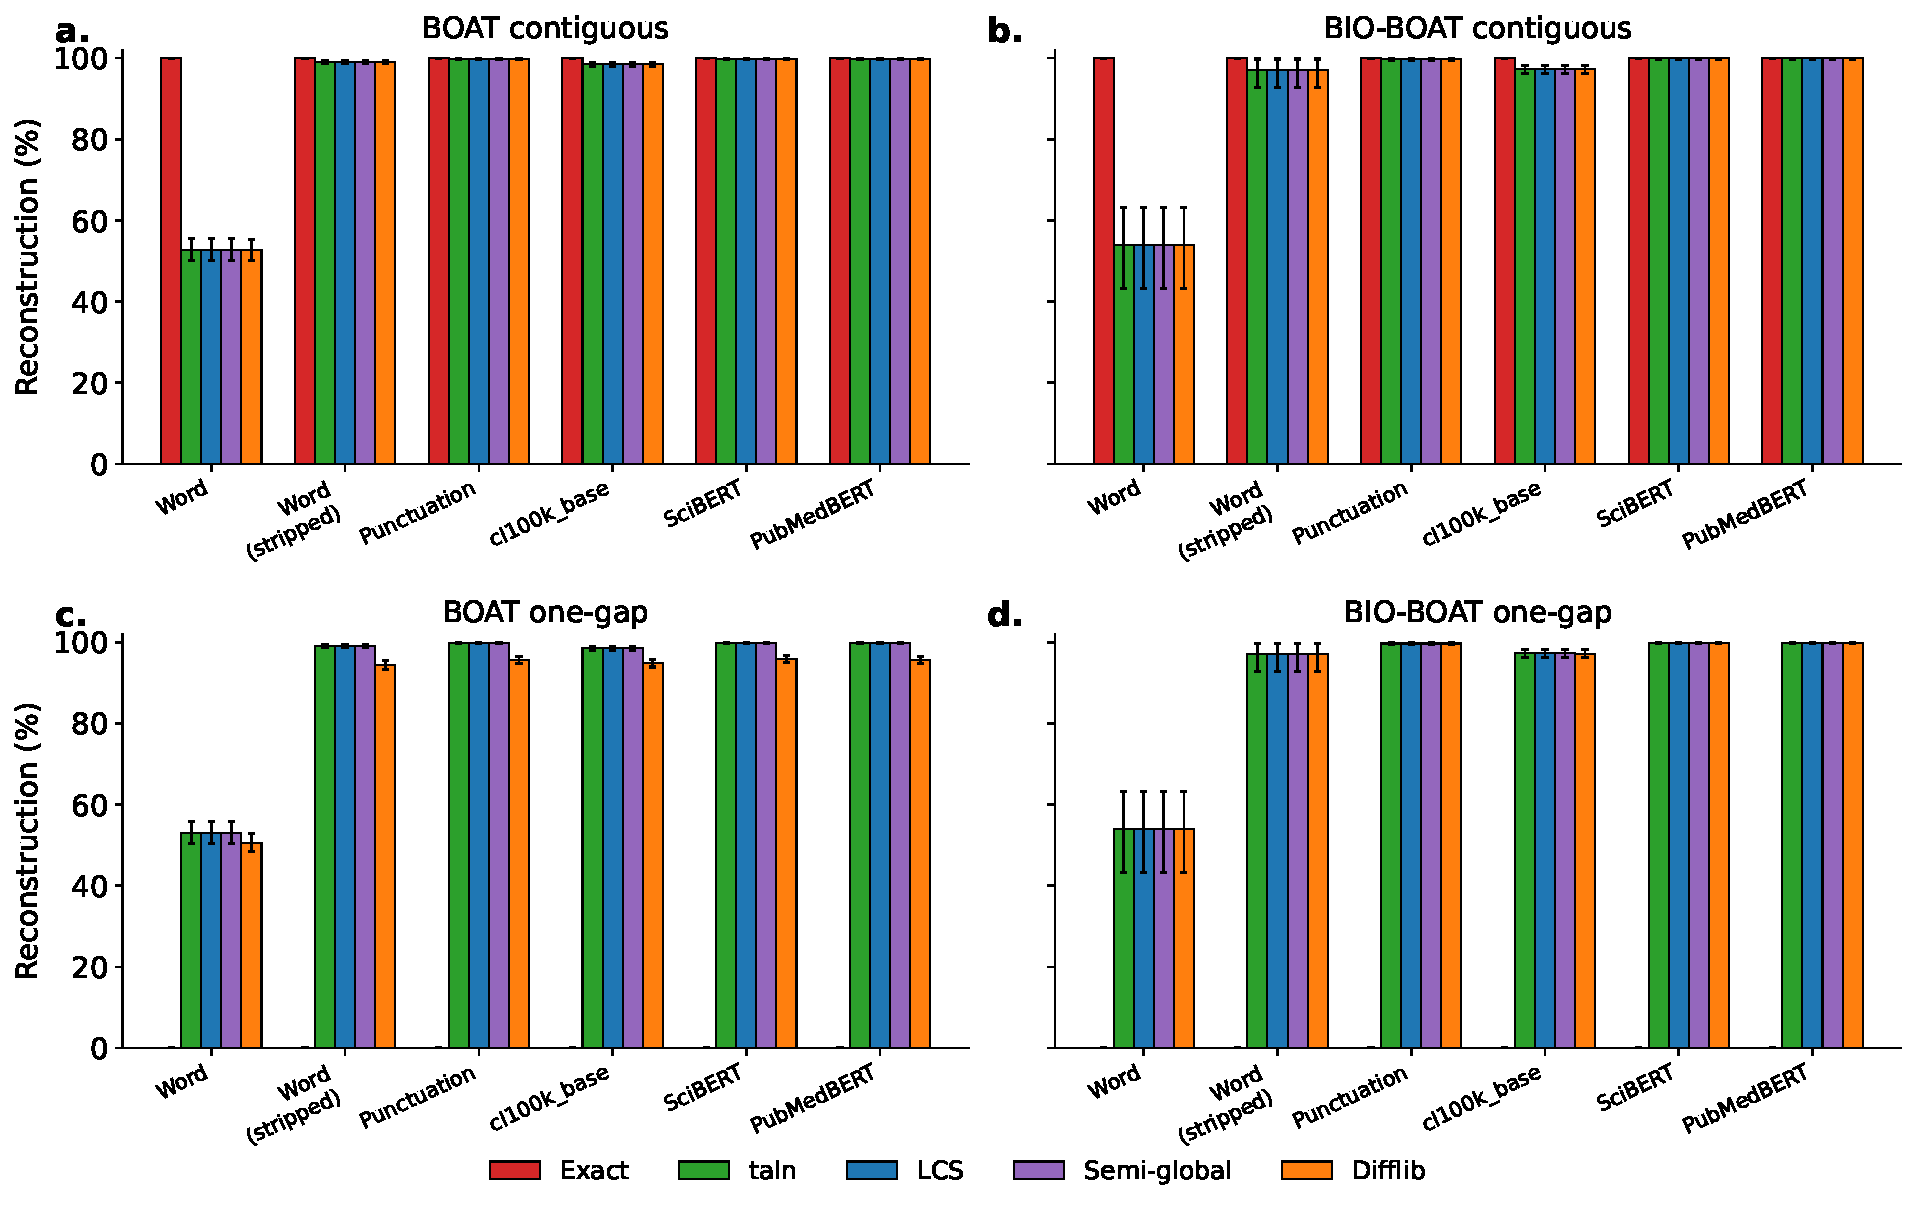
\includegraphics[width=0.75\linewidth]{../../shared/figures/reconstruction_accuracy.pdf}
    \caption{\textbf{Reconstruction accuracy across methods and tokenizers.} Held-out reconstruction for exact string matching, \texttt{taln}, LCS, semi-global alignment, and \texttt{difflib} under six tokenizers, with document-clustered 95\% confidence intervals. \textbf{a.} \texttt{BOAT} contiguous (n=4,313). \textbf{b.} \texttt{BIO-BOAT} contiguous (n=1,259). \textbf{c.} \texttt{BOAT} one-gap (n=4,284). \textbf{d.} \texttt{BIO-BOAT} one-gap (n=1,259). Exact string matching does not depend on the tokenizer and is shown at every position.}
    \label{fig:match_acc_all}
\end{figure*}

\begin{figure*}[h]
    \centering
    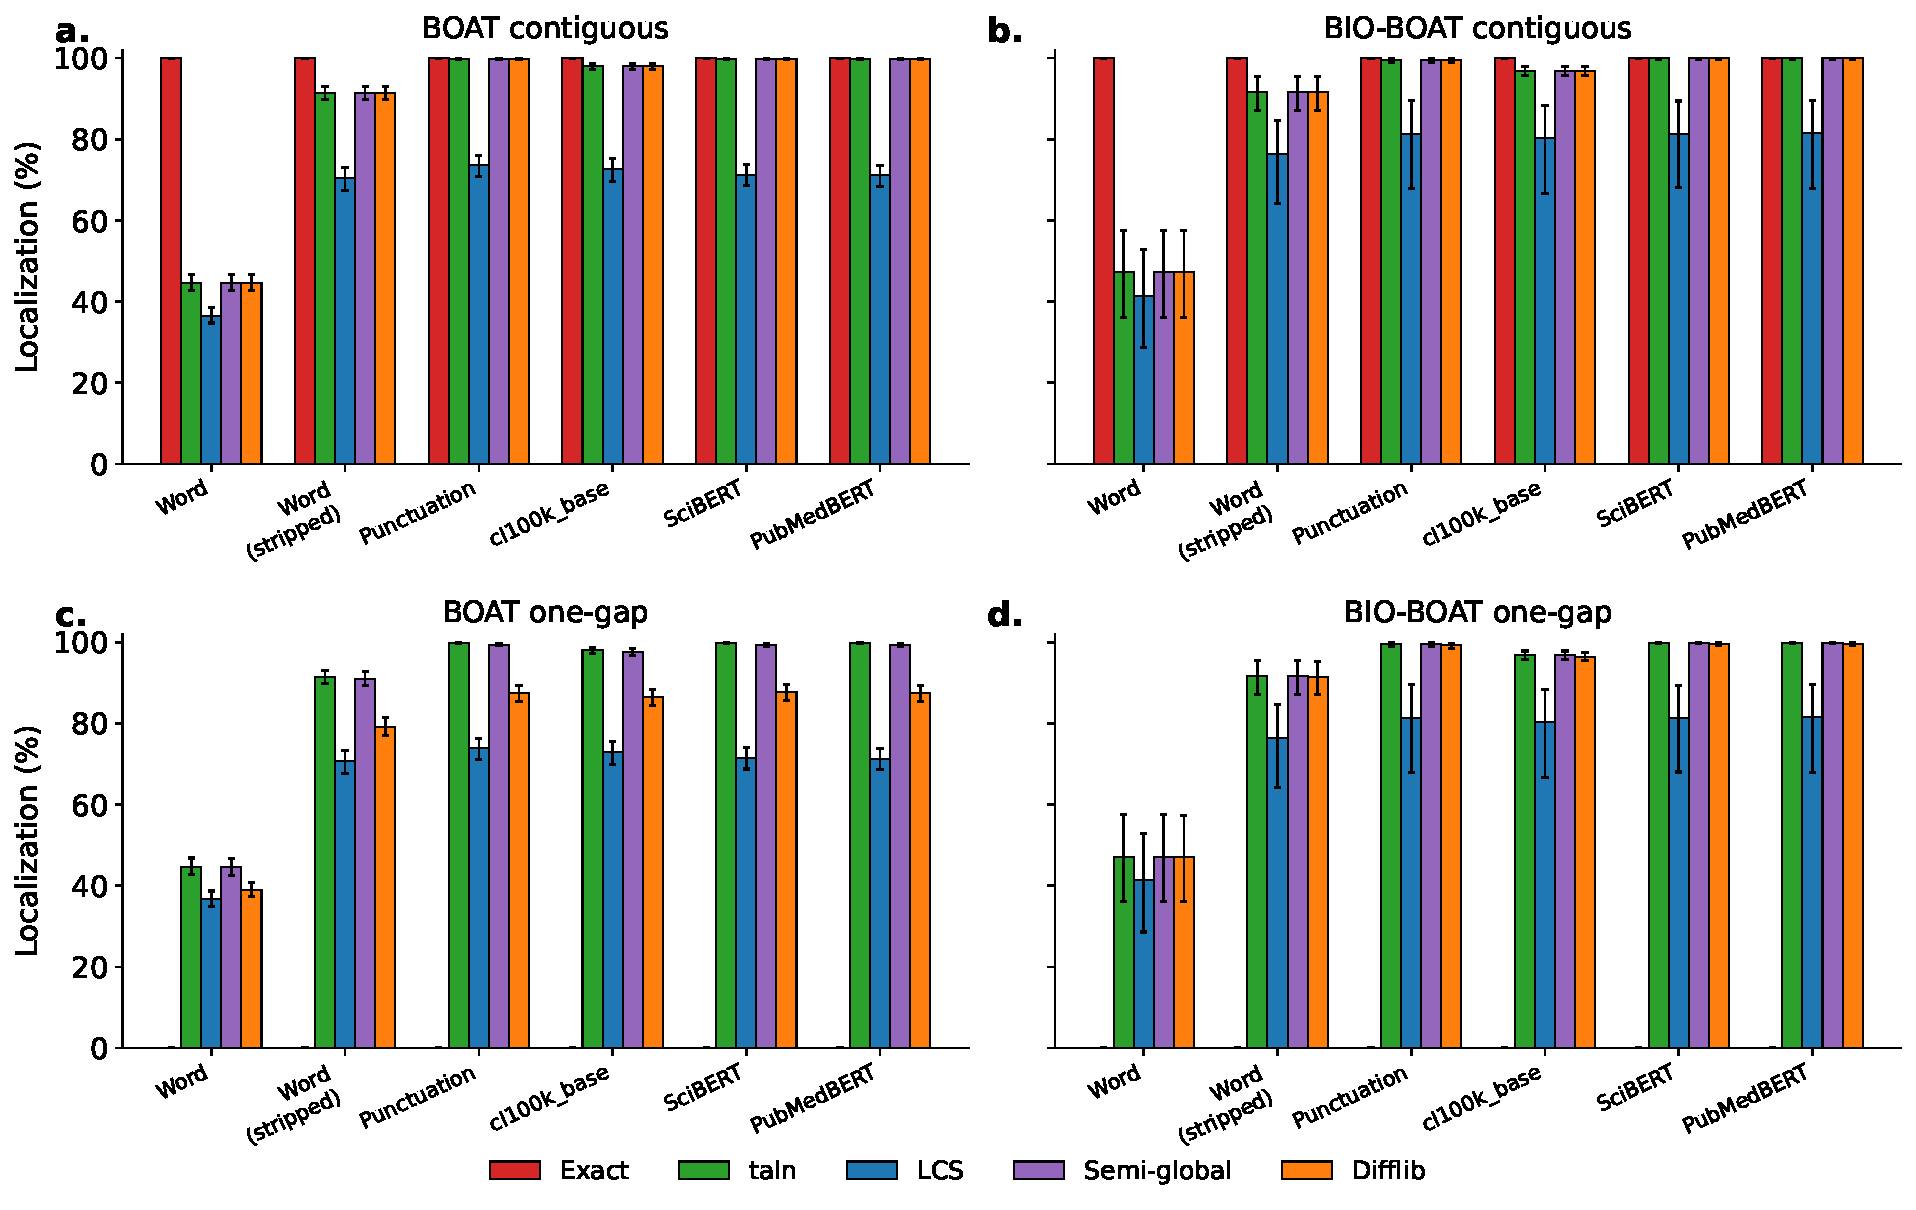
\includegraphics[width=0.75\linewidth]{../../shared/figures/localization_accuracy.pdf}
    \caption{\textbf{Localization accuracy across methods and tokenizers.} Held-out localization for the same methods, tokenizers, and conditions as Supplementary Figure S1, with document-clustered 95\% confidence intervals. Localization requires a reconstructing alignment to start and end at a correct location in the original source.}
    \label{fig:loc_acc_all}
\end{figure*}



% \clearpage
% \newpage

% \section{Supplementary Note}
% Sequence alignment has a long history of algorithm development in computational linguistics and genomics. Classical methods include text matching algorithms like Knuth–Morris–Pratt \citep{KnuthMorrisPratt1977} for exact substring detection, dynamic-programming aligners for gapped and approximate matches \citep{needlemanwunsch1970, smithwaterman1981}, pseudoalignment methods for transcriptomics \citep{Bray2016kallisto}, and genome rearrangement models for studying structural variation \citep{hannenhallipevzner1999permutations, tesler2002grimm}. Although these tools are used in different domains, they share a common goal: relate one sequence to another through alignment.

Here we develop a unified framework, that makes this connection explicit. We treat every alignment problem as the search for a function $f$ mapping positions in one sequence to positions in another under a chosen set of constraints, inspired by the formalism put forth in \citep{schwartz2007seqanneal}. Contiguous matches, ordered subsequences, pseudoalignments, and rearrangements all appear as special cases distinguished only by which constraints on $f$ are enforced or relaxed.

This framework reveals a natural hierarchy. By comparing constraint families, we obtain a partially ordered set over alignment classes, ordered from the most restrictive (exact substring matching) to the least (arbitrary realignments). From this structure, ordered alignment naturally falls out as the most permissive alignment strategy, for text, under practical computational constraints (number of alignments). It sits above classical (contiguous) text alignment, and below partial permutation alignment. In the main text, we realize this alignment strategy, with subword token sequences, to verify the existence of text extracted by large language models. 

% \newpage
\section{Results}
Text alignment is the process of finding a map between two sequences, the target and the source. If such a map exists, then the target is said to fully align to the source---such as \texttt{CAT} aligning to \texttt{SCATTER}. 

This example is intuitive and simple but makes two implicit assumptions. The first is that the alignment is contiguous---that every aligned character must directly follow the previous. The second is that the objects being aligned are characters themselves (instead of other features like groups of characters, $n$-grams). 

By formalizing text alignment and making these assumptions explicit, we can more easily compare complex alignment algorithms. The differences between them get reduced to choices of the alignment objects (tokens) and the constraints on the alignment itself. With this formalization we find that contiguous text alignment is a special case of pseudoalignment.

\subsection{Ordered alignment}
Suppose we have a source sequence of characters  $\mathbf{s} = (s_1,\dots,s_n)$ and a target sequence of characters $\mathbf{t} = (t_1,\dots,t_m)$. An order-preserving alignment map is a function $f : \{1,\dots,m\} \to \{1,\dots,n\},$ which maps each position of the target to a position in the source, subject to an order constraint on $f$. 

If we only care that the alignment is ordered (permitting gaps) then the constraint family is the set of functions $f(1) < f(2) < \dots < f(m)$, $s_{f(j)} = t_j$, $ \text{for all } j.$ If such an $f$ exists, then $\mathbf{t}$ appears in $\mathbf{s}$ as a (possibly non-contiguous) ordered subsequence.  
The set of all maps is given by the set of functions:
\begin{align}
\mathcal{E}_{\mathrm{MA}}(\mathbf{t},\mathbf{s}) = \big\{ f : f(1)<\cdots<f(m),\; s_{f(j)} = t_j\ \forall j \big\}.
\end{align}


\paragraph{Example: Character alignment.}
Consider $s=\texttt{SCATTER}$ and $t=\texttt{CAT}$. The positions of \texttt{C} and \texttt{A} in $s$ are fixed to $2$ and $3$, while the final \texttt{T} may align to either $s_4$ or $s_5$.

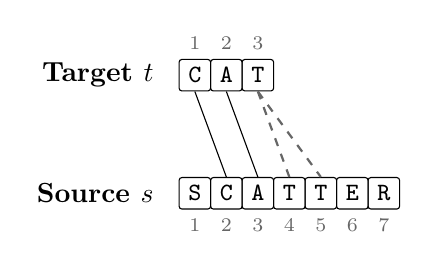
\begin{tikzpicture}[
  char/.style={
    draw, rounded corners=1pt,
    minimum width=4mm, minimum height=4mm,
    inner sep=0pt,
    font=\ttfamily\small, align=center
  },
  idx/.style={font=\scriptsize, text=black!60},
  match/.style={dashed, thick, black!60}
]
\def\xstep{0.4}

% --- Target t (top) ---
\node[anchor=east, font=\bfseries] at (0,0) {Target $t$};
\foreach \c [count=\i] in
  {C,A,T}
{
  \node[char] (t\i) at (\xstep*\i,0) {\c};
  \node[idx] at ([yshift=2mm]t\i.north) {\i};
}

% --- Source s (bottom) ---
\node[anchor=east, font=\bfseries] at (0,-1.5) {Source $s$};
\foreach \c [count=\i] in
  {S,C,A,T,T,E,R}
{
  \node[char] (s\i) at (\xstep*\i,-1.5) {\c};
  \node[idx] at ([yshift=-2mm]s\i.south) {\i};
}

% --- Alignment lines ---
\draw (t1.south) -- (s2.north);
\draw (t2.south) -- (s3.north);
\draw[match] (t3.south) -- (s4.north);
\draw[match] (t3.south) -- (s5.north);


\end{tikzpicture}\\
The ambiguity in the final \texttt{T} leads to multiple alignments $\mathcal{E}_{\mathrm{MA}}(\mathbf{t},\mathbf{s}) = \big\{ f : (f(1),f(2),f(3)) \in \{(2,3,4),(2,3,5)\} \big\},$ whereas the simple example above (contiguous alignment) permits only one valid map.

% \newpage
\subsection{General alignment}
With the example above in mind, we now put forth a framework for classifying alignment methods. Let $\Sigma$ be a character alphabet, let $V$ be a vocabulary of tokens, and let
$\tau : \Sigma^* \to V^*$ be a tokenizer that maps sequences of characters to sequences of tokens.
For a source $S \in \Sigma^*$ and a target $T \in \Sigma^*$, define
\begin{align}
\tau(S) &= \mathbf{s} = (s_1,\dots,s_n), \\
\tau(T) &= \mathbf{t} = (t_1,\dots,t_m).
\end{align}
Given a source $\mathbf{s}$ and target $\mathbf{t}$, an alignment map is a function
\begin{align}
f : \{1,\dots,m\} \to \{1,\dots,n\},
\end{align}
which maps each position of the target to a position in the source.

Different alignment tasks impose different requirements on how $f$ may behave.
We refer to any collection of such requirements as a constraint family $\mathcal{C}$. Typical constraints include monotonicity, contiguity, distance bounds, membership conditions, and cardinality properties of $f$. A map $f$ is injective if distinct target positions never map to the same source position (no duplication), and surjective if every source position is used by at least one target position (no deletion). A bijective map is both injective and surjective and represents a one-to-one correspondence between source and target positions.

Given a constraint family $\mathcal{C}$, the set of all valid maps of
$\mathbf{t}$ into $\mathbf{s}$ is
\begin{align}
\mathcal{E}_{\mathcal{C}}(\mathbf{t},\mathbf{s})
=
\big\{
f : f \text{ satisfies } \mathcal{C} \text{ and } s_{f(j)} = t_j \;\; \forall j
\big\},
\end{align}
with the equality condition replaced or relaxed as appropriate for the specific alignment class. Thus each alignment problem corresponds to specifying a constraint family $\mathcal{C}$ and then determining the structure of $\mathcal{E}_{\mathcal{C}}(\mathbf{t},\mathbf{s})$.

We now describe several common tokenizers and constraint families on the function $f$. Each family defines a corresponding set of valid maps. Each example assumes a given alphabet $\Sigma$ with $S,T\in\Sigma^*$. Unless otherwise specified, the tokenizer $\tau$ is the character tokenizer, $\mathbf{t} = \tau_{\mathrm{char}}(T)$, $\mathbf{s} = \tau_{\mathrm{char}}(S).$

\paragraph{Contiguous alignment.}
The strongest constraint on the alignment map $f$ is contiguity: the target must appear as a contiguous sequence in the source. The constraint family and map set are
\begin{align}
\mathcal{C}_{\mathrm{CA}}
&=
\{\, f : f(j{+}1) = f(j)+1 \ \text{for all } j \,\}, \\
\mathcal{E}_{\mathrm{CA}}(\mathbf{t},\mathbf{s})
&=
\big\{
f : f \in \mathcal{C}_{\mathrm{CA}},\;
s_{f(j)} = t_j \ \forall j
\big\}.
\end{align}
This class recovers exact substring search: each token of the target must match the source at consecutive positions. An example of this is classical string search \citep{KnuthMorrisPratt1977}. The contiguity constraint forces $f$ to be injective. In the worst case, the number of valid maps is linear in the input size when all tokens are identical ($|\mathcal{E}_{\mathrm{CA}}(\mathbf{t},\mathbf{s})| \le n-m+1$).

\paragraph{Ordered alignment.}
Relaxing contiguity gives ordered, non-contiguous matches. As previously discussed, the constraint family and map set are
\begin{align}
\mathcal{C}_{\mathrm{OA}} &= \{\, f : f(1)<f(2)<\dots<f(m) \,\}, \\
\mathcal{E}_{\mathrm{OA}}(\mathbf{t},\mathbf{s}) &= \big\{f : f \in \mathcal{C}_{\mathrm{OA}},\;s_{f(j)} = t_j \ \forall j\big\}.
\end{align}
This class captures ordered subsequences, allowing gaps but preserving the order of tokens. Examples include classical dynamic-programming techniques to find the longest common subsequence (LCS) \citep{hirschberg1975lcs}. The number of alignments in the worst case is achieved when all tokens match $|\mathcal{E}_{\mathrm{OA}}(\mathbf{t},\mathbf{s})| \le \binom{n}{m} \approx \frac{n^m}{m!}$.

Classical global and local aligners (Needleman–Wunsch \citep{needlemanwunsch1970}, Smith–Waterman \citep{smithwaterman1981}, Wagner–Fischer \citep{wagnerfischer1974cost}) operate in this same constraint family, but select a single map by maximizing a scoring function with match rewards and gap penalties instead of returning all valid maps.
\begin{align}
\text{Score}(f)
=
\sum_{j=1}^m S(s_{f(j)},t_j) \;-\; \text{gap penalties}.
\end{align}

\paragraph{Partial permutation alignment.}
Removing monotonicity but preserving one-to-one matching yields partial permutation alignment: each target position selects a distinct source position, but order is unrestricted and the source need not be fully covered. The constraint family and map set are
\begin{align}
\mathcal{C}_{\mathrm{PPA}}
&=
\{\, f : f \text{ injective} \,\}, \\
\mathcal{E}_{\mathrm{PPA}}(\mathbf{t},\mathbf{s})
&=
\big\{
f : f \in \mathcal{C}_{\mathrm{PPA}},\;
s_{f(j)} = t_j \ \forall j
\big\}.
\end{align}
This class models permutation-like reorderings for the common setting where the target may be shorter than the source. The familiar bijective permutation case is recovered when $m=n$, where every source position is used exactly once. When $m\le n$, the worst case number of valid partial permutation alignments is achieved when all tokens match, $|\mathcal{E}_{\mathrm{PPA}}(\mathbf{t},\mathbf{s})| \le \frac{n!}{(n-m)!}$, which reduces to $n!$ when $m=n$.

If $f$ is surjective but not injective, then every source position is used by at least one target position, and some may be used repeatedly. Without order constraints, this class corresponds to many-to-one assignments (partitions of the target indices).

\paragraph{General rearrangement alignment.}
Dropping both the order constraint and cardinality constraint allows arbitrary reorderings, including duplications or deletions. Here duplication corresponds to non-injective $f$ (two targets mapping to the same source position), and deletion corresponds to non-surjective $f$ (some source positions not hit by any target). The constraint family and map set are
\begin{align}
\mathcal{C}_{\mathrm{RA}}
&=
\{\, f : f \text{ arbitrary} \,\}, \\
\mathcal{E}_{\mathrm{RA}}(\mathbf{t},\mathbf{s}) &= \big\{ f : s_{f(j)} = t_j \ \forall j \big\}.
\end{align}
This class captures structural processes such as large-scale genome rearrangements and other arbitrary reorderings with duplications and deletions. In the worst case, the number of alignments is achieved when every target token matches every source position ($|\mathcal{E}_{\mathrm{RA}}(\mathbf{t},\mathbf{s})| \le n^m$.)

If we instead use a $k$-mer tokenizer, letting $\mathbf{u}=\tau_k(S)$ and $\mathbf{v}=\tau_k(T)$, this same constraint family underlies pseudoalignment \citep{Bray2016kallisto, Melsted2021, Sullivan2025}: a map $f$ is allowed to be arbitrary, and practical algorithms retain only membership information (whether each $k$-mer of $\mathbf{u}$ appears somewhere in $\mathbf{v}$) rather than the full map $f$.

\paragraph{Approximate alignment.}
Any of the classes above can be combined with a relaxed matching rule. Instead of requiring exact equality $s_{f(j)} = t_j$, we allow mismatches under a distance threshold $d(s_{f(j)},t_j) \le \varepsilon$ for all $j$. Here $\tau$ may be the character tokenizer or a higher-level tokenizer (e.g.\ words). This relaxation yields mismatch-tolerant variants of contiguous, ordered, or rearrangement alignment. Examples include Hamming-distance--based matching algorithms.

\subsection{A partial order of alignment}

The alignment classes above differ only in the constraints they impose on the
map function~$f$. Stronger constraint families admit fewer maps,
while weaker families admit more. This creates a natural hierarchy. Formally, for two constraint families $\mathcal{C}_1$ and $\mathcal{C}_2$, we
write $\mathcal{C}_1 \preceq \mathcal{C}_2$ if any map that satisfies
$\mathcal{C}_1$ also satisfies $\mathcal{C}_2$. Equivalently, $\mathcal{E}_{\mathcal{C}_1}(\mathbf{x},\mathbf{y}) \subseteq \mathcal{E}_{\mathcal{C}_2}(\mathbf{x},\mathbf{y})$ for all $\mathbf{x},\mathbf{y}.$

\begin{theorem}[Alignment classes form a partial order]
Let $\mathsf{C}$ be the set of alignment classes defined by constraint
families. The relation $\preceq$ on $\mathsf{C}$ is a partial order: it is
reflexive, antisymmetric, and transitive. Moreover, the classes introduced
above satisfy $ \mathcal{C}_{\mathrm{CA}} \;\preceq\; \mathcal{C}_{\mathrm{OA}} \;\preceq\; \mathcal{C}_{\mathrm{PPA}} \;\preceq\; \mathcal{C}_{\mathrm{RA}}.$
\end{theorem}

\begin{proof}
Reflexivity follows because every map set is contained within itself: $\mathcal{E}_{\mathcal{C}}(X,Y) \subseteq \mathcal{E}_{\mathcal{C}}(X,Y).$ For antisymmetry, if $\mathcal{C}_1 \preceq \mathcal{C}_2$ and
$\mathcal{C}_2 \preceq \mathcal{C}_1$, then
$
\mathcal{E}_{\mathcal{C}_1}(X,Y) = \mathcal{E}_{\mathcal{C}_2}(X,Y)$, for all $X,Y$ so the two classes impose the same constraints on $f$. Transitivity is immediate from the transitivity of set inclusion.

For the chain, each step relaxes one structural condition. Contiguous alignment requires $f(j{+}1)=f(j)+1$; ordered alignment keeps strict order but allows gaps; partial permutation alignment removes the monotonicity requirement but still forbids reuse of source positions; and the rearrangement class imposes no restrictions on $f$. Each relaxation enlarges the corresponding map set, establishing the chain.
\end{proof}

\subsection{Alignment ambiguity}
Different constraint families yield map sets of different sizes. Strict classes often admit a unique map or none at all, while weaker classes may admit many.  Ambiguity arises whenever the source contains repeated tokens or when positional restrictions are relaxed. Note that as a consequence of the chain more constrained mappings have fewer alignments: $|\mathcal{E}_{\mathrm{CA}}(\mathbf{t},\mathbf{s})| \;\le\; |\mathcal{E}_{\mathrm{OA}}(\mathbf{t},\mathbf{s})|\;\le\; |\mathcal{E}_{\mathrm{PPA}}(\mathbf{t},\mathbf{s})| \;\le\; |\mathcal{E}_{\mathrm{RA}}(\mathbf{t},\mathbf{s})|$.

For example, for $s=\texttt{DAD}$ and $t=\texttt{ADD}$, the positions matching each \texttt{D} in $t$ may map to either occurrence of \texttt{D} in $s$. Under ordered alignment, no map exists, but under partial permutation or rearrangement constraints there are multiple valid choices for $f$. Thus relaxing constraints not only enlarges the map set but also increases the number of admissible mappings; a larger map set corresponds to greater alignment ambiguity.

\section{Discussion}
Historically, alignment methods in computational linguistics and genomics focused on developing algorithms for a specific task. These algorithms were optimized independently for biological sequences or natural language text. As a result, similarities between these algorithms remained silo-ed in different journals and software tools.

We unify these approaches by framing alignment as a map $f$ between token sequences, with methods primarily distinguished by the constraints imposed on this map. Under this view, any alignment method is defined by three choices: a tokenizer, a constraint family on the map, and a selection rule for choosing an alignment.

This framing makes relationships between methods explicit. For example,  classical text alignment imposes stricter constraints when mapping an extracted piece of text to a passage than genomics pseudoalignment does when mapping a sequencing read to a transcriptome. These constraints implicitly define a trade-off between computational complexity and alignment ambiguity. Once an algorithm is placed within a constraint family, its possible relaxations or tightenings become clear, along with their effects on ambiguity and computational cost. This allows scientists to reason about speed, memory usage, and alignment multiplicity prior to implementation.

By organizing alignment methods in this way, we connect two disciplines that have largely evolved independently. This connection enables mathematical and algorithmic ideas developed in genomics to be reused in natural language processing, and vice versa (Table~\ref{tab:cfam}). Indexing strategies, hashing schemes, and alignment selection rules can be transferred across domains within a shared formal framework. In this work, we combine algorithms and computational techniques from genomics \citep{Bray2016kallisto, Melsted2021, Sullivan2025} with tokenization and alignment selection ideas from natural language processing \citep{hirschberg1975lcs,sennrich2016neuralmachinetranslationrare}. The alignment tool discussed in the manuscript (\texttt{taln}) emerges naturally from this framework. It uses ordered alignment over subword tokens to balance alignment flexibility with computational efficiency.

\newpage
\section{Simple alignment examples}

We list short examples that illustrate how different constraint families
$\mathcal{C}$ behave on small strings. For a source $\mathbf{x}$ and target
$\mathbf{y}$, we describe whether maps exist under each class and, when
helpful, the number of valid maps.

\paragraph{Contiguous alignment.}
Requires $f(j{+}1)=f(j)+1$.
\begin{itemize}
    \item $\mathbf{x}=\texttt{SCATTER}$, $\mathbf{y}=\texttt{CAT}$:
    one valid map $\{(2,3,4)\}$.
    \item $\mathbf{x}=\texttt{ABCDE}$, $\mathbf{y}=\texttt{ACE}$:
    no contiguous map.
\end{itemize}

\paragraph{Ordered alignment.}
Requires $f(1)<\cdots<f(m)$.
\begin{itemize}
    \item $\mathbf{x}=\texttt{ABCDE}$, $\mathbf{y}=\texttt{ACE}$:
    one map $\{(1,3,5)\}$, which is ordered but non-contiguous.
    \item $\mathbf{x}=\texttt{DAD}$, $\mathbf{y}=\texttt{ADD}$:
    no map.
\end{itemize}

\paragraph{Partial permutation alignment}
Here $f$ is injective and order is unrestricted.
\begin{itemize}
    \item $\mathbf{x}=\texttt{ABC}$, $\mathbf{y}=\texttt{CBA}$:
    one map, the reversal $\{(3,2,1)\}$.
    \item $\mathbf{x}=\texttt{ABCDE}$, $\mathbf{y}=\texttt{CEA}$:
    one partial permutation map $\{(3,5,1)\}$, which is neither contiguous nor ordered.
    \item $\mathbf{x}=\texttt{ABA}$, $\mathbf{y}=\texttt{BAA}$:
    two maps $\{(2,1,3), (2,3,1)\}$.
\end{itemize}
The bijective permutation case is recovered when the source and target have the same length. A different relaxation, where $f$ is surjective but not injective, corresponds to sequence partitioning.

\paragraph{General rearrangement alignment.}
Here $f$ is arbitrary (not required to be bijective nor injective).
\begin{itemize}
    \item $\mathbf{x}=\texttt{CAT}$, $\mathbf{y}=\texttt{CAAT}$:
    duplication $(1,2,2,3)$, since the single \texttt{A} in $\mathbf{x}$ must
    be used twice.
    \item $\mathbf{x}=\texttt{GGA}$, $\mathbf{y}=\texttt{GA}$:
    deletion $\{(1,3),(2,3)\}$, since one of the \texttt{G} positions in
    $\mathbf{x}$ is not used.
\end{itemize}

With a $k$-mer tokenizer, this rearrangement class underlies
pseudoalignment. With $k{=}2$,
\begin{itemize}
    \item $\mathbf{x}=\texttt{GATTACA}$ yields 2-mers
          $\mathbf{u}=\texttt{GA,AT,TT,TA,AC,CA}$,
    \item $\mathbf{y}=\texttt{TTA}$ yields 2-mers
          $\mathbf{v}=\texttt{TT,TA}$.
\end{itemize}
An arbitrary map $f$ with $u_{f(j)} = v_j$ exists (both \texttt{TT} and \texttt{TA} occur in $\mathbf{u}$), so $\mathbf{y}$ is pseudoaligned to $\mathbf{x}$ with the alignment $\{(3,4)\}$.

\newpage
\begin{sidewaystable}[t!]
\centering
\footnotesize
\setlength{\tabcolsep}{4pt}
\renewcommand{\arraystretch}{1.4}
\caption{Alignment classes defined by structural constraints on the map
function $f$.}
\begin{tabular}{l p{4.0cm} p{5.0cm} p{5.0cm}}
\toprule
\textbf{Name} &
\textbf{Constraint family $\mathcal{C}$} &
\textbf{Map set $\mathcal{E}_{\mathcal{C}}(\mathbf{t},\mathbf{s})$} &
\textbf{Classical algorithms} \\
\midrule

\textbf{Contiguous alignment} &
$\{ f : f(j{+}1)=f(j)+1 \}$ &
$\{ f : f \in \mathcal{C}_{\mathrm{CA}},\; s_{f(j)}=t_j\ \forall j \}$ &
KMP, Boyer--Moore; exact substring search \\
\midrule

\textbf{Ordered alignment} &
$\{ f : f(1)<\dots<f(m) \}$ &
$\{ f : f \in \mathcal{C}_{\mathrm{OA}},\; s_{f(j)}=t_j\ \forall j \}$ &
LCS, edit distance, Needleman--Wunsch, Smith--Waterman \\
\midrule

\textbf{Partial permutation alignment} &
$\{ f : f \text{ injective} \}$ &
$\{ f : f \in \mathcal{C}_{\mathrm{PPA}},\; s_{f(j)} = t_j\ \forall j \}$ &
Partial rearrangement models; permutation distance when $m=n$ \\
\midrule

\textbf{General rearrangement} &
$\{ f : f \text{ arbitrary} \}$ &
$\{ f : s_{f(j)} = t_j\ \forall j \}$ &
Genome rearrangements, V(D)J recombination; pseudoalignment (with $k$-mers) \\
\bottomrule
\end{tabular}
\label{tab:cfam}
\end{sidewaystable}


\clearpage
\newpage


\bibliographystyle{unsrtnat}
\bibliography{../../shared/references}
\end{document}
